\chapter*{Проектирование системы}
\addcontentsline{toc}{chapter}{Проектирование системы}

\section*{Концептуальный дизайн}
\addcontentsline{toc}{section}{Концептуальный дизайн}

\subsection*{Концептуальная модель системы в нотации IDEF0}
\addcontentsline{toc}{subsection}{Концептуальная модель системы в нотации IDEF0}

Для создания функциональной модели портала, отражающей его основные функции и потоки информации наиболее наглядно использовать нотацию IDEF0. 
На рисунке 1 приведена концептуальная модель системы. На рисунке 2 представлена декомпозиция функциональной модели системы.

\begin{figure}[h!]
    \centering
    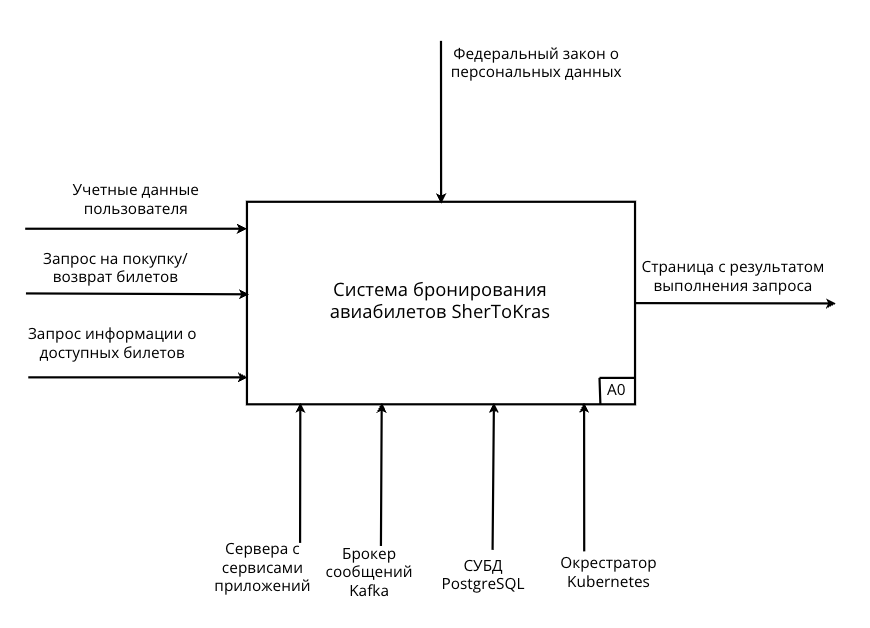
\includegraphics[width=1.05\textwidth]{../images/idef0-0.png}
    \caption{Концептуальная модель в нотации IDEF0}
    \label{images:algorithm}
\end{figure}

\begin{figure}[H]
    \centering
    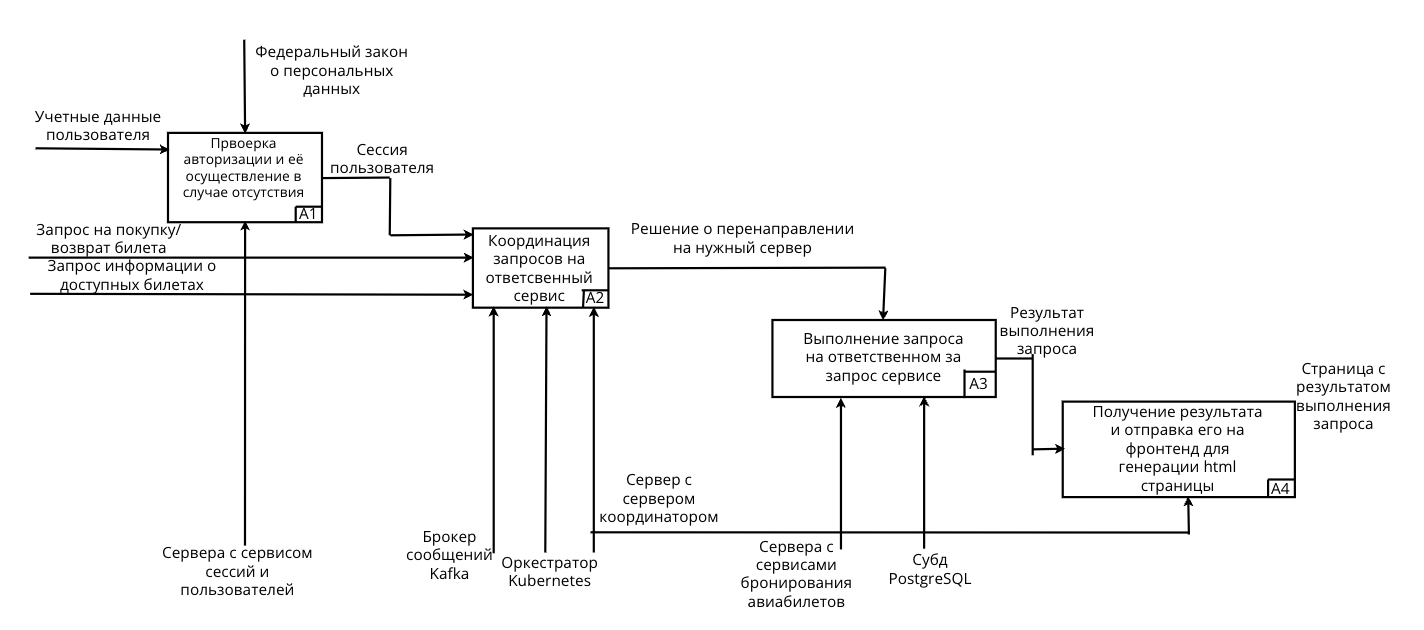
\includegraphics[width=1.05\textwidth]{../images/idef0-1.jpg}
    \caption{Детализированная концептуальная модель в нотации IDEF0}
    \label{images:algorithm}
\end{figure}

\section*{Сценарии функционирования системы}
\addcontentsline{toc}{section}{Сценарии функционирования системы}

\textbf{Регистрация пользователя}
\begin{enumerate}
	\item Пользователь нажимает на кнопку <<Зарегистрироваться>> в интерфейсе.
	\item Пользователь перенаправляется на страницу, которая содержит поля для заполнения его данных.
	\item Пользователь вводит данные в форму и для завершения регистрации нажимает на кнопку <<Зарегистрироваться>>, тем самым подтверждая верность своих данных, а также согласие на их обработку и хранение.
	\item Если пользователь с введенным для регистрации логином, почтой или номером телефона уже существует, то клиент получает сообщение об ошибке. При успешной регистрации клиент попадает на страниицу для просмотра авиабилетов.
\end{enumerate}

\textbf{Авторизация клиента}
\begin{enumerate}
	\item Пользователь нажимает на кнопку <<Авторизоваться>> в интерфейсе.
	\item Пользователь перенаправляется на страницу авторизации, которая содержит поля для заполнения логина и пароля.
	\item Пользователь завершает работу с формой авторизации нажатием кнопки <<Войти>>.
	\item При обнаружении ошибки в данных, пользователь получает сообщение об ошибке; при совпадении данных с записью в базе данных аккаунтов пользователь получает доступ к системе и перенаправляется на страниицу для просмотра авиабилетов.
\end{enumerate}

\textbf{Поиск и просмотр билетов по заданным фильтрам пользователем}
\begin{enumerate}
    \item Функциональность доступна как авторизованным, так и неавторизованным пользователям.
    \item Пользователь вводит параметры поиска в форму:
    \begin{itemize}
        \item пункт отправления;
        \item пункт назначения;
        \item дата рейса;
        \item количество пассажиров;
        \item класс обслуживания (эконом, бизнес и т.д.).
    \end{itemize}
    \item После ввода параметров пользователь инициирует поиск.
    \item Результаты поиска отображаются на той же странице в виде набора карточек рейсов.
    \item Каждая карточка содержит полную информацию о рейсе: маршрут, дата и время отправления и прибытия, длительность, стоимость и доступность мест.
    \item Для каждого найденного рейса предоставляется кнопка \textit{«Забронировать»}, при нажатии на которую пользователь переходит на страницу оформления бронирования.
\end{enumerate}

\textbf{Покупка билета}
\begin{enumerate}
    \item После того как пользователь выполнил поиск рейсов, он нажимает на кнопку \textit{«Забронировать»}, расположенную напротив выбранного рейса.
    \item Пользователь перенаправляется на отдельную страницу с детальной информацией по выбранному рейсу, включая обновлённую цену и условия.
    \item В нижней части страницы отображается кнопка \textit{«Оплатить»}.
    \item После нажатия на кнопку \textit{«Оплатить»}, пользователь перенаправляется на страницу платёжного шлюза CloudPayments.
    \item Пользователь выбирает способ оплаты, вводит данные и подтверждает транзакцию.
    \item В случае успешной оплаты и положительного ответа от банка, пользователь попадает на страницу постобработки.
    \item На этой странице отображается уведомление: \textbf{«Билет успешно забронирован»}.
    \item Пользователю предоставляются две кнопки:
    \begin{itemize}
        \item \textit{«Мои бронирования»} — переводит пользователя на страницу активных бронирований.
        \item \textit{«На главную»} — возвращает пользователя на главную страницу для повторного поиска рейсов.
    \end{itemize}
\end{enumerate}

\textbf{Возврат купленного билета}
\begin{enumerate}
	\item Для просмотра купленных билетов пользователь переходит на страницу <<Билеты>>, нажимая соответсвующую кнопку в выезжающем боковом меню.
	\item Пользователь попадает на страницу, на которой видит все свои купленные и сданные билеты.
	\item У каждого купленного билета есть кнопка <<Сдать билет>>, на которую нажимает пользователь.
	\item В появившемся модальном окно подтверждения с подробной информацией о выбранном билете пользователь нажимает на кнопку <<Подтвердить>>.
  \item Пользователь видит измененный статус билета на <<Билет сдан>> и обновленный баланс бонусного счета.
\end{enumerate}

\textbf{Просмотр пользователем личного кабинета}
\begin{enumerate}
    \item Пользователь нажимает на вкладку «Личный кабинет» в нижней панели интерфейса.
    \item Система проверяет, авторизован ли пользователь:
    \begin{itemize}
        \item Если пользователь неавторизован, происходит перенаправление на страницу с формой регистрации/входа.
        \item Если пользователь авторизован, осуществляется переход на страницу личного кабинета.
    \end{itemize}
    \item На странице личного кабинета отображается персональная информация пользователя:
    \begin{itemize}
        \item Электронная почта и город.
        \item Список разделов: профиль, бонусная программа, мои бронирования, данные пассажира, поддержка, контакты, правила и соглашения, гарантии, настройки.
    \end{itemize}
    \item Пользователь может перейти в любой из представленных разделов, нажав на соответствующий пункт.
\end{enumerate}

\textbf{Просмотр активных бронирований пользователм}
\begin{enumerate}
    \item Пользователь, находясь в личном кабинете, нажимает на вкладку \textit{«Мои бронирования»}.
    \item Система проверяет, авторизован ли пользователь:
    \begin{itemize}
        \item Если пользователь неавторизован, доступ к разделу невозможен (по умолчанию пользователь не может попасть в личный кабинет).
        \item Если пользователь авторизован, происходит переход на страницу активных бронирований.
    \end{itemize}
    \item На странице отображается список всех активных бронирований пользователя:
    \begin{itemize}
        \item Каждое бронирование представлено в виде отдельной карточки с информацией о рейсе (маршрут, дата, пассажиры, статус и т.д.).
        \item Рядом с каждым бронированием присутствует кнопка \textit{«Отменить бронирование»}, позволяющая отменить бронь.
    \end{itemize}
    \item Если у пользователя отсутствуют активные бронирования, на экране отображается водяной знак с текстом \textit{«Нет активных бронирований»}.
\end{enumerate}

\section*{Диаграммы прецедентов}
\addcontentsline{toc}{section}{Диаграммы прецедентов}

Для детальной разработки портала используется унифицированный язык моделирования UML. 
В системе выделены 2 роли: администратор и пользователь (авторизованный и неавторизованный). 
На рисунках 4-3 представлены диаграммы прецедентов для выделенных ролей и описаны сценарии функционирования наиболее значимых прецедентов.

\begin{figure}[H]
    \centering
    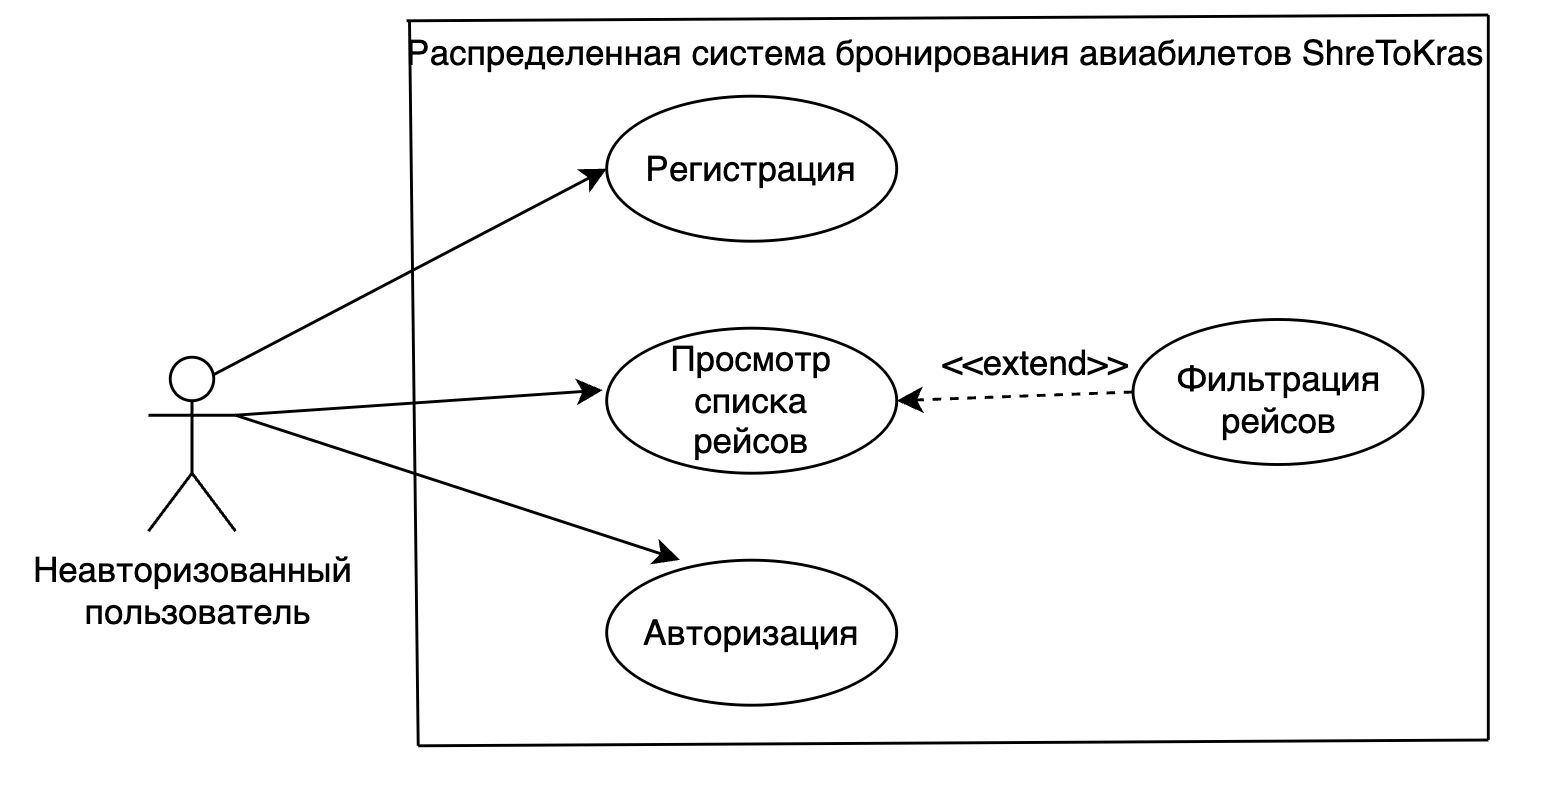
\includegraphics[width=1.05\textwidth]{../images/unauthorized.jpg}
    \caption{Диаграмма прецедентов с точки зрения Неавторизованного пользователя}
    \label{images:algorithm}
\end{figure}


\section*{Спецификация сценария <<регистрация пользователя>>}
\addcontentsline{toc}{section}{Спецификация сценария <<регистрация пользователя>>}

\textbf{Нормальный ход сценария}
\begin{longtable}{|p{8cm}|p{8cm}|}
    \hline
    \textbf{Действие актера} & \textbf{Откик системы} \\
    \endfirsthead
    \hline
    \textbf{Действие актера} & \textbf{Отклик системы} \\
    \hline
    \endhead

    \hline
    Пользователь нажимает кнопку "Регистрация" на стартовой странице &
    Система предоставляет пользователю форму для регистрации, в которой нужно заполнить фамилию, имя, логин, пароль, номер телефона, электронную почту \\
    
    \hline
    Пользователь заполняет поля формы (фамилию, имя, логин, пароль, номер телефона, электронную почту), согласно необходимому формату, и нажимает кнопку "Зарегистрироваться" &
    Данные пользователя регистрируются в системе. Пользователь перенаправляется на главную страницу портала с формой для поиска рейсов. \\
    \hline
\end{longtable}

\textbf{Альтернативный ход сценария}
\begin{longtable}{|p{8cm}|p{8cm}|}
    \hline
    \textbf{Действие актера} & \textbf{Откик системы} \\
    \endhead

    \hline
    Пользователь нажимает кнопку "Регистрация" на стартовой странице &
    Система предоставляет пользователю форму для регистрации, в которой нужно заполнить фамилию, имя, логин, пароль, номер телефона, электронную почту \\

    \hline
    Пользователь заполняет поля формы (фамилию, имя, логин, пароль, номер телефона, электронную почту) и нажимает кнопку "Зарегистрироваться", но в одном из них введенные данные, не соотвествуют требуемому формату &
    На странице регистрации под формой появляется сообщение о неверном формате заполненных данных \\
    \hline
\end{longtable}

\begin{figure}[H]
    \centering
    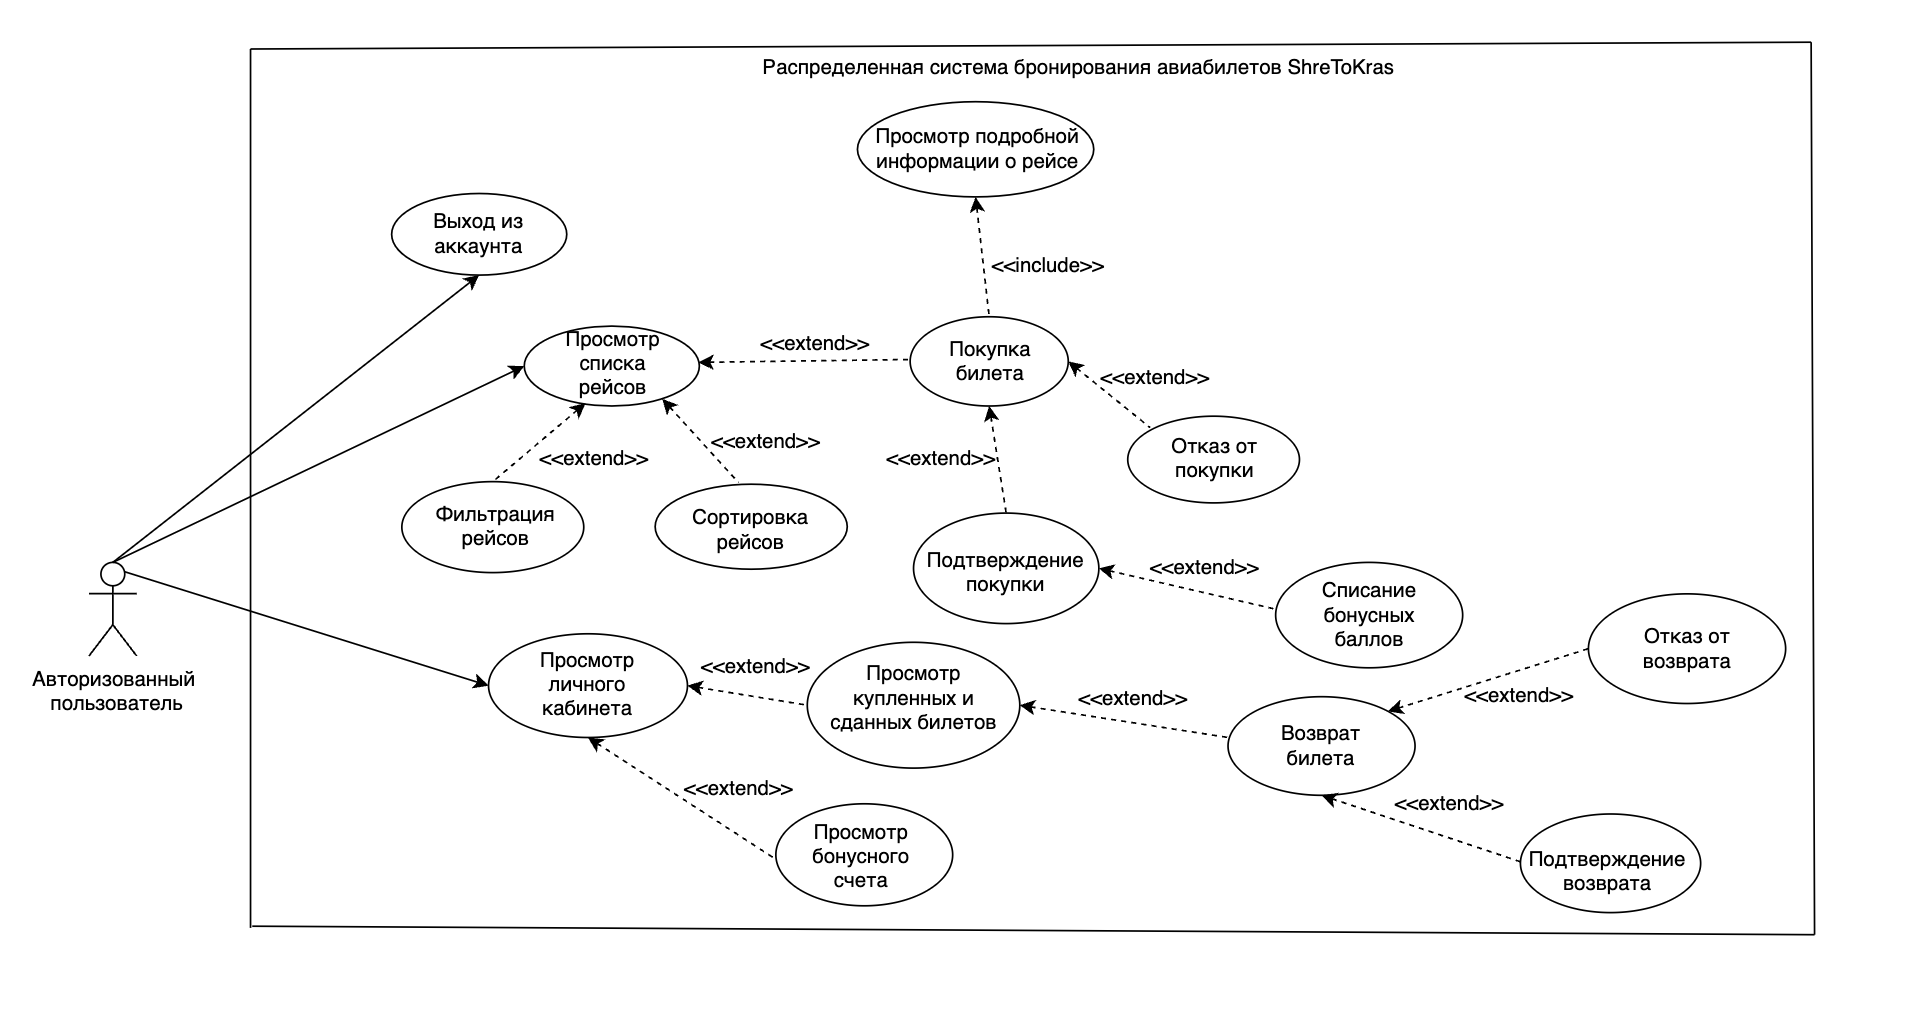
\includegraphics[width=1.05\textwidth]{../images/authorized.jpg}
    \caption{Диаграмма прецедентов с точки зрения Авторизованного пользователя}
    \label{images:algorithm}
\end{figure}

\section*{Спецификация сценария <<авторизация пользователя>>}
\addcontentsline{toc}{section}{Спецификация сценария <<авторизация пользователя>>}

\textbf{Нормальный ход сценария}
\begin{longtable}{|p{8cm}|p{8cm}|}
    \hline
    \textbf{Действие актера} & \textbf{Откик системы} \\
    \endhead

    \hline
    Пользователь нажимает кнопку "Авторизация" на стартовой странице &
    Система предоставляет пользователю форму для авторизации, в которой нужно заполнить логин, пароль \\

    \hline
    Пользователь заполняет поля формы (логин, пароль) и нажимает кнопку "Войти" &
    Система проверяет правильность введенных пользователем данных и, если данные правильные, перенаправляет пользователя на главную страницу портала с формой для поиска рейсов \\
    \hline
\end{longtable}

\textbf{Альтернативный ход сценария}
\begin{longtable}{|p{8cm}|p{8cm}|}
    \hline
    \textbf{Действие актера} & \textbf{Откик системы} \\
    \endhead

    \hline 
    Пользователь нажимает кнопку "Авторизация" на стартовой странице &
    Система предоставляет пользователю форму для авторизации, в которой нужно заполнить логин, пароль, номер телефона, электронную почту \\

    \hline Пользователь заполняет поля формы и нажимает кнопку "Войти", но при этом преднамеренно или нет совершает ошибку при вводе логина и пароля &
    Система отказывает в доступе и на странице авторизации под формой появляется сообщение о том, что пользователь с данной комбинацией логина и пароля не найден \\
    \hline
\end{longtable}

\begin{figure}[H]
    \centering
    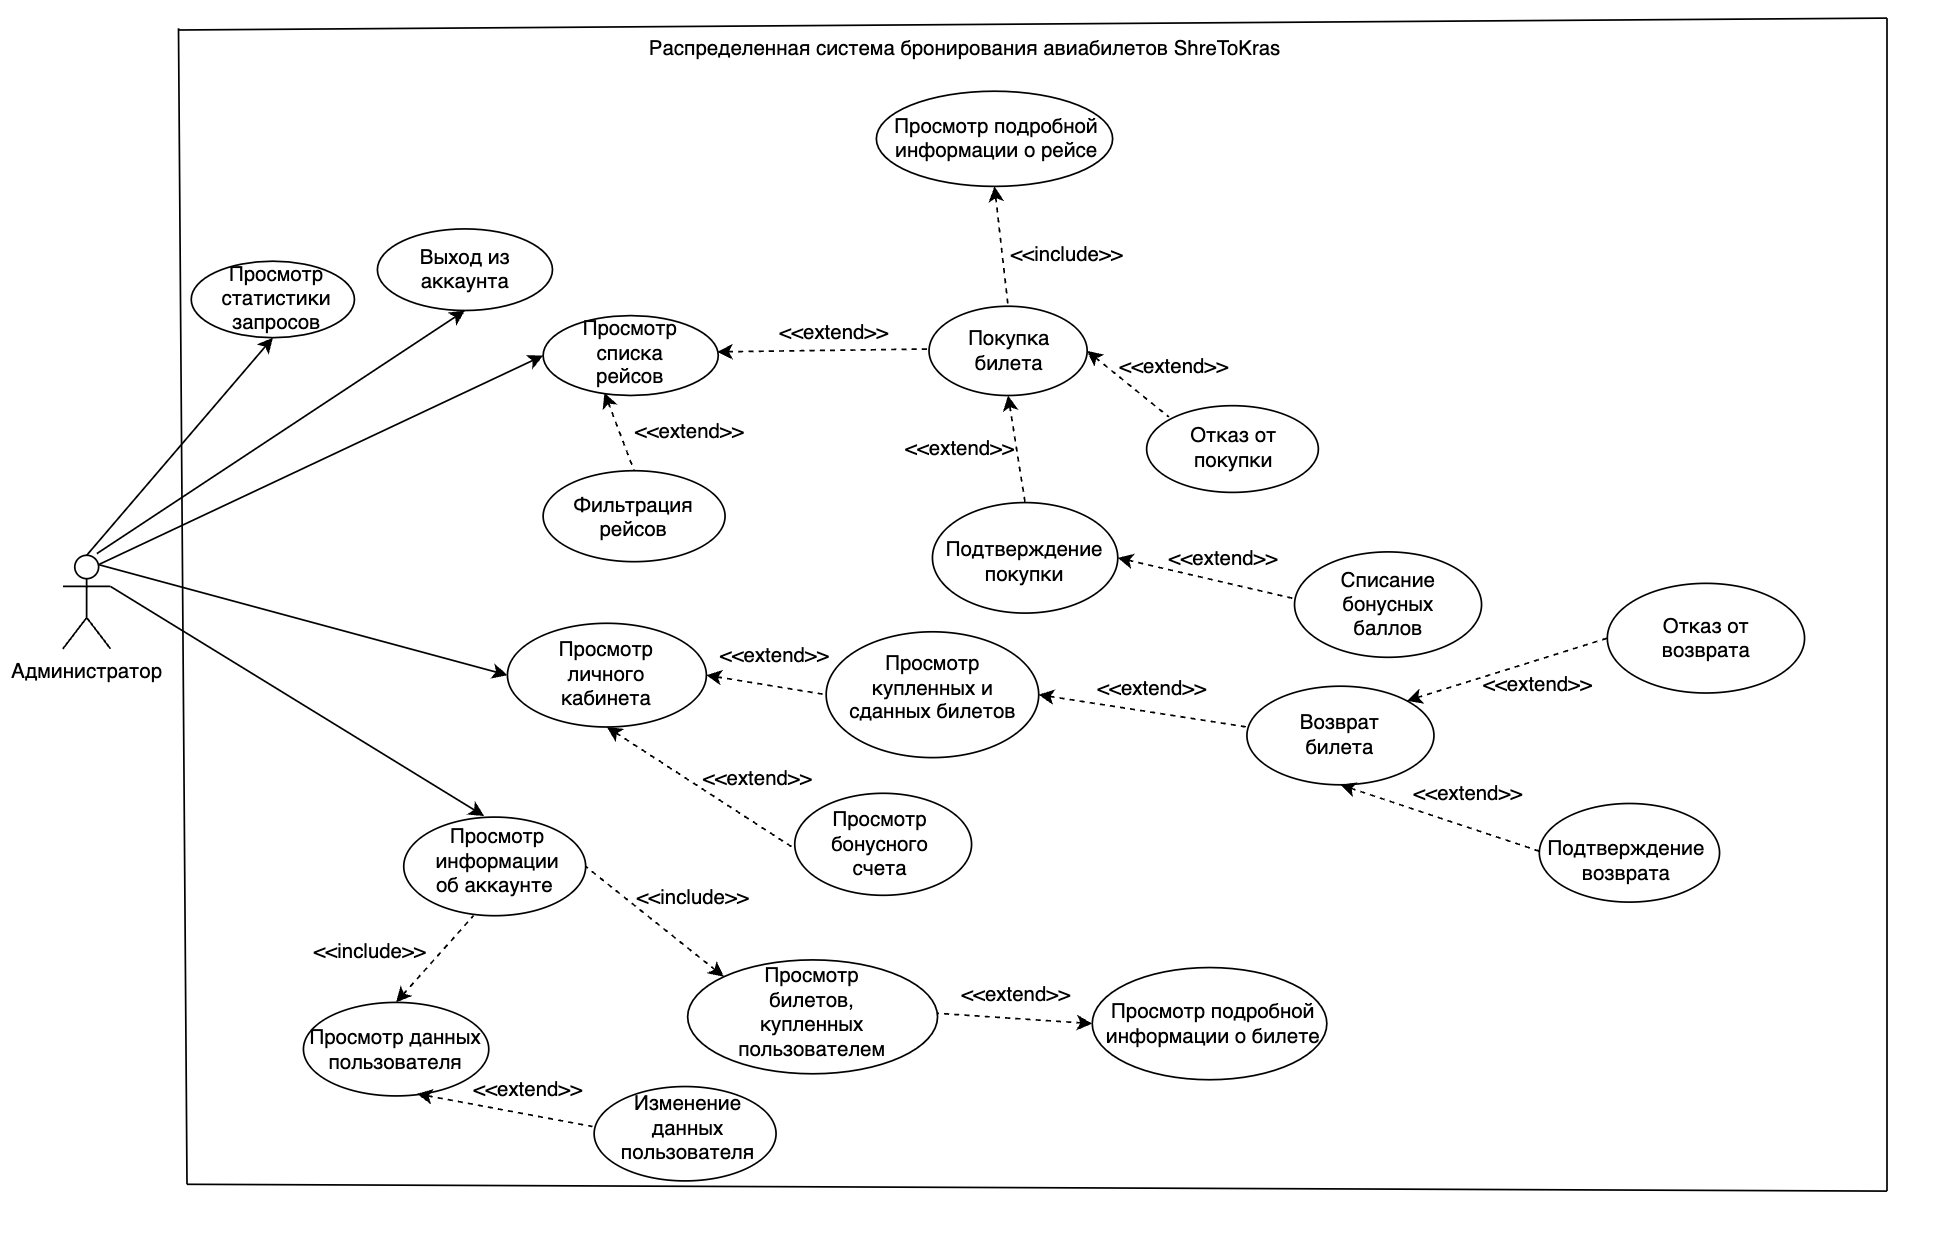
\includegraphics[width=1.05\textwidth]{../images/admin.jpg}
    \caption{Диаграмма прецедентов с точки зрения Администратора}
    \label{images:algorithm}
\end{figure}

\subsubsection*{Спецификация сценария <<покупка билета>>}
\addcontentsline{toc}{section}{Спецификация сценария <<покупка билета>>}

\textbf{Нормальный ход сценария.}
\begin{longtable}{|p{8cm}|p{8cm}|}
    \hline
    \textbf{Действие актера} & \textbf{Откик системы} \\
    \endhead
    
    \hline
    После успешной авторизации пользователь попадает на главную страницу портала, на которой представлена форма для поиска рейсов. Форма содержит в себе несколько полей для задания параметров поискового запроса рейсов
    (номер полета, аэропорт отправления/прибытия, время вылета/прилета, минимальная/максимальная цена). Пользователь должен заполнить как минимум одно из полей формы, чтобы система могла сформировать поисковый запрос рейсов. &
    Система формирует запрос на получение списка рейсов по заданным параметрам, передаёт его в сервис поиска рейсов, получает список соответствующих рейсов и возвращает данные, которые на клиентской стороне отображаются в виде карточек с информацией о рейсе и кнопкой для покупки. \\

    \hline
    Пользователь нажимает на кнопку "Забронировать" в карточке рейса для бронирования билета. & 
    Система делает запрос на проверку наличия билетов по данному рейсу, после чего пользователь перенаправляется на страницу с подробной информацией о рейсе и кнопкой "Оплатить".
    Предваритеьно система проверяет, есть ли у пользователя бонусные баллы, и в зависимости от этого под информацией о рейсе появляется switch-кнопка "Списать бонусные баллы". \\
    
    \hline
    Пользователь имеет возможность нажать на кнопку "Использовать бонусные баллы" & 
    Система обновляет финальную стоитмость билета на странице с подробной информацией о билете в соответсвие с информацией о используемых пользователем бонусных баллах. \\
    
    \hline
    Пользователь нажимает кнопку "Оплатить" для совершения оплаты билета. & 
    Система перенаправляет пользователя на страницу с оплатой через платежный шлюз. \\
    
    \hline 
    Пользователь вводит данные своей карты и нажимает кнопку "Оплатить"
    & Платежный шлюз отправляет запрос в соответствующий банк для подтверждения транзакции. \\
    
    \hline
    Пользователь перенаправляется на страницу платежного шлюза для ожидания завершения транзакции.
    & После успешного завершения транзакции система перенаправляет пользователя на страницу с рейсами и отображает модальное окно с информацией о том, что рейс забронирован и сколько бонусных баллов было зачислено на бонусный счет пользователя. \\
    \hline
\end{longtable}

\newpage

\textbf{Альтернативный ход сценрия.}
\begin{longtable}{|p{8cm}|p{8cm}|}
    \hline
    \textbf{Действие актера} & \textbf{Откик системы} \\
    \endhead

    \hline
    После успешной авторизации пользователь попадает на главную страницу портала на которой представлена форма для поиска рейсов. Форма содержит в себе несколько полей для задания параметров поискового запроса рейсов
    (номер полета, аэропорт отправления/прибытия, время вылета/прилета, минимальная/максимальная цена). Пользователь должен заполнить как минимум одно из полей формы, чтобы система могла сформировать поисковый запрос рейсов. &
    Система формирует запрос на получение списка рейсов по заданным параметрам, передаёт его в сервис поиска рейсов, но по данному запросу не находится ни одного рейса. Система отправляет сообщение об этом на фронтент, и перед пользователем появляется сообщение "По вашему запросу рейсов не найдено" \\
    \hline
\end{longtable}

\newpage

\textbf{Альтернативный ход сценария.}
\begin{longtable}{|p{8cm}|p{8cm}|}
    \hline
    \textbf{Действие актера} & \textbf{Откик системы} \\
    \endhead
    
    \hline
    После успешной авторизации пользователь попадает на главную страницу портала на которой представлена форма для поиска рейсов. Форма содержит в себе несколько полей для задания параметров поискового запроса рейсов
    (номер полета, аэропорт отправления/прибытия, время вылета/прилета, минимальная/максимальная цена). Пользователь должен заполнить как минимум одно из полей формы, чтобы система могла сформировать поисковый запрос рейсов. &
    Система формирует запрос на получение списка рейсов по заданным параметрам, передаёт его в сервис поиска рейсов, получает список соответствующих рейсов и возвращает данные, которые на клиентской стороне отображаются в виде карточек с информацией о рейсе и кнопкой для покупки. \\
    
    \hline
    Пользователь нажимает на кнопку "Забронировать" в карточке рейса для бронирования билета. & 
    Система делает запрос на проверку наличия билетов по данному рейсу, после чего пользователь перенаправляется на страницу с подробной информацией о рейсе и кнопкой "Оплатить".
    Предваритеьно система проверяет, есть ли у пользователя бонусные баллы, и в зависимости от этого под информацией о рейсе появляется switch-кнопка "Списать бонусные баллы". \\
    
    \hline
    Пользователь имеет возможность нажать на кнопку "Использовать бонусные баллы", если у него ненулевой бонусный баланс. &
    Система обновляет финальную стоимость билета на странице с подробной информацией о билете в соответствии с информацией о используемых пользователем бонусных баллах. \\
    
    \hline
    Пользователь нажимает кнопку “Оплатить” на странице с подробной информацией о билете, но не авторизован. Это может произойти, например, если срок действия пользовательской сессии истёк, куки были удалены или произошёл сбой в хранении токена авторизации. &
    Система перенаправляет пользователя на страницу авторизации. \\
    
    \hline
    Пользователь вводит данные для авторизации (логин и пароль) и нажимает кнопку "Войти". &
    Система проверяет правильность введенных данных пользователя. Если данные правильные, перенаправляет пользователя на страницу с оплатой через платежный шлюз. \\
    
    \hline
    Пользователь вводит данные своей карты и нажимает кнопку "Оплатить". &
    Платежный шлюз отправляет запрос в соответствующий банк для подтверждения транзакции. \\
    
    \hline
    Платежный шлюз получает подтверждение от банка и завершает операцию оплаты. &
    Система перенаправляет пользователя на страницу с рейсами и отображает модальное окно с информацией о том, что рейс забронирован и сколько бонусных баллов было зачислено на бонусный счет пользователя. \\ 
    \hline
\end{longtable}

\section*{Логический дизайн}
\addcontentsline{toc}{section}{Логический дизайн}

\subsection*{Диаграммы классов}
\addcontentsline{toc}{subsection}{Диаграммы классов}
Иерархии классов для разработки серверных приложений представлены в виде диаграммы классов:
\begin{itemize}
    \item сервиса рейсов --  на рисунке 6;
    \item сервиса билетов --  на рисунке 7;
    \item сервиса сессий и пользователей --  на рисунке 8;
    \item сервиса программы лояльности --  на рисунке 9;
    \item сервиса-координатора --  на рисунке 10;
    \item сервиса оплаты --  на рисунке 11;
    \item сервиса статистики --  на рисунке 12.
\end{itemize}

\begin{figure}[H]
    \centering
    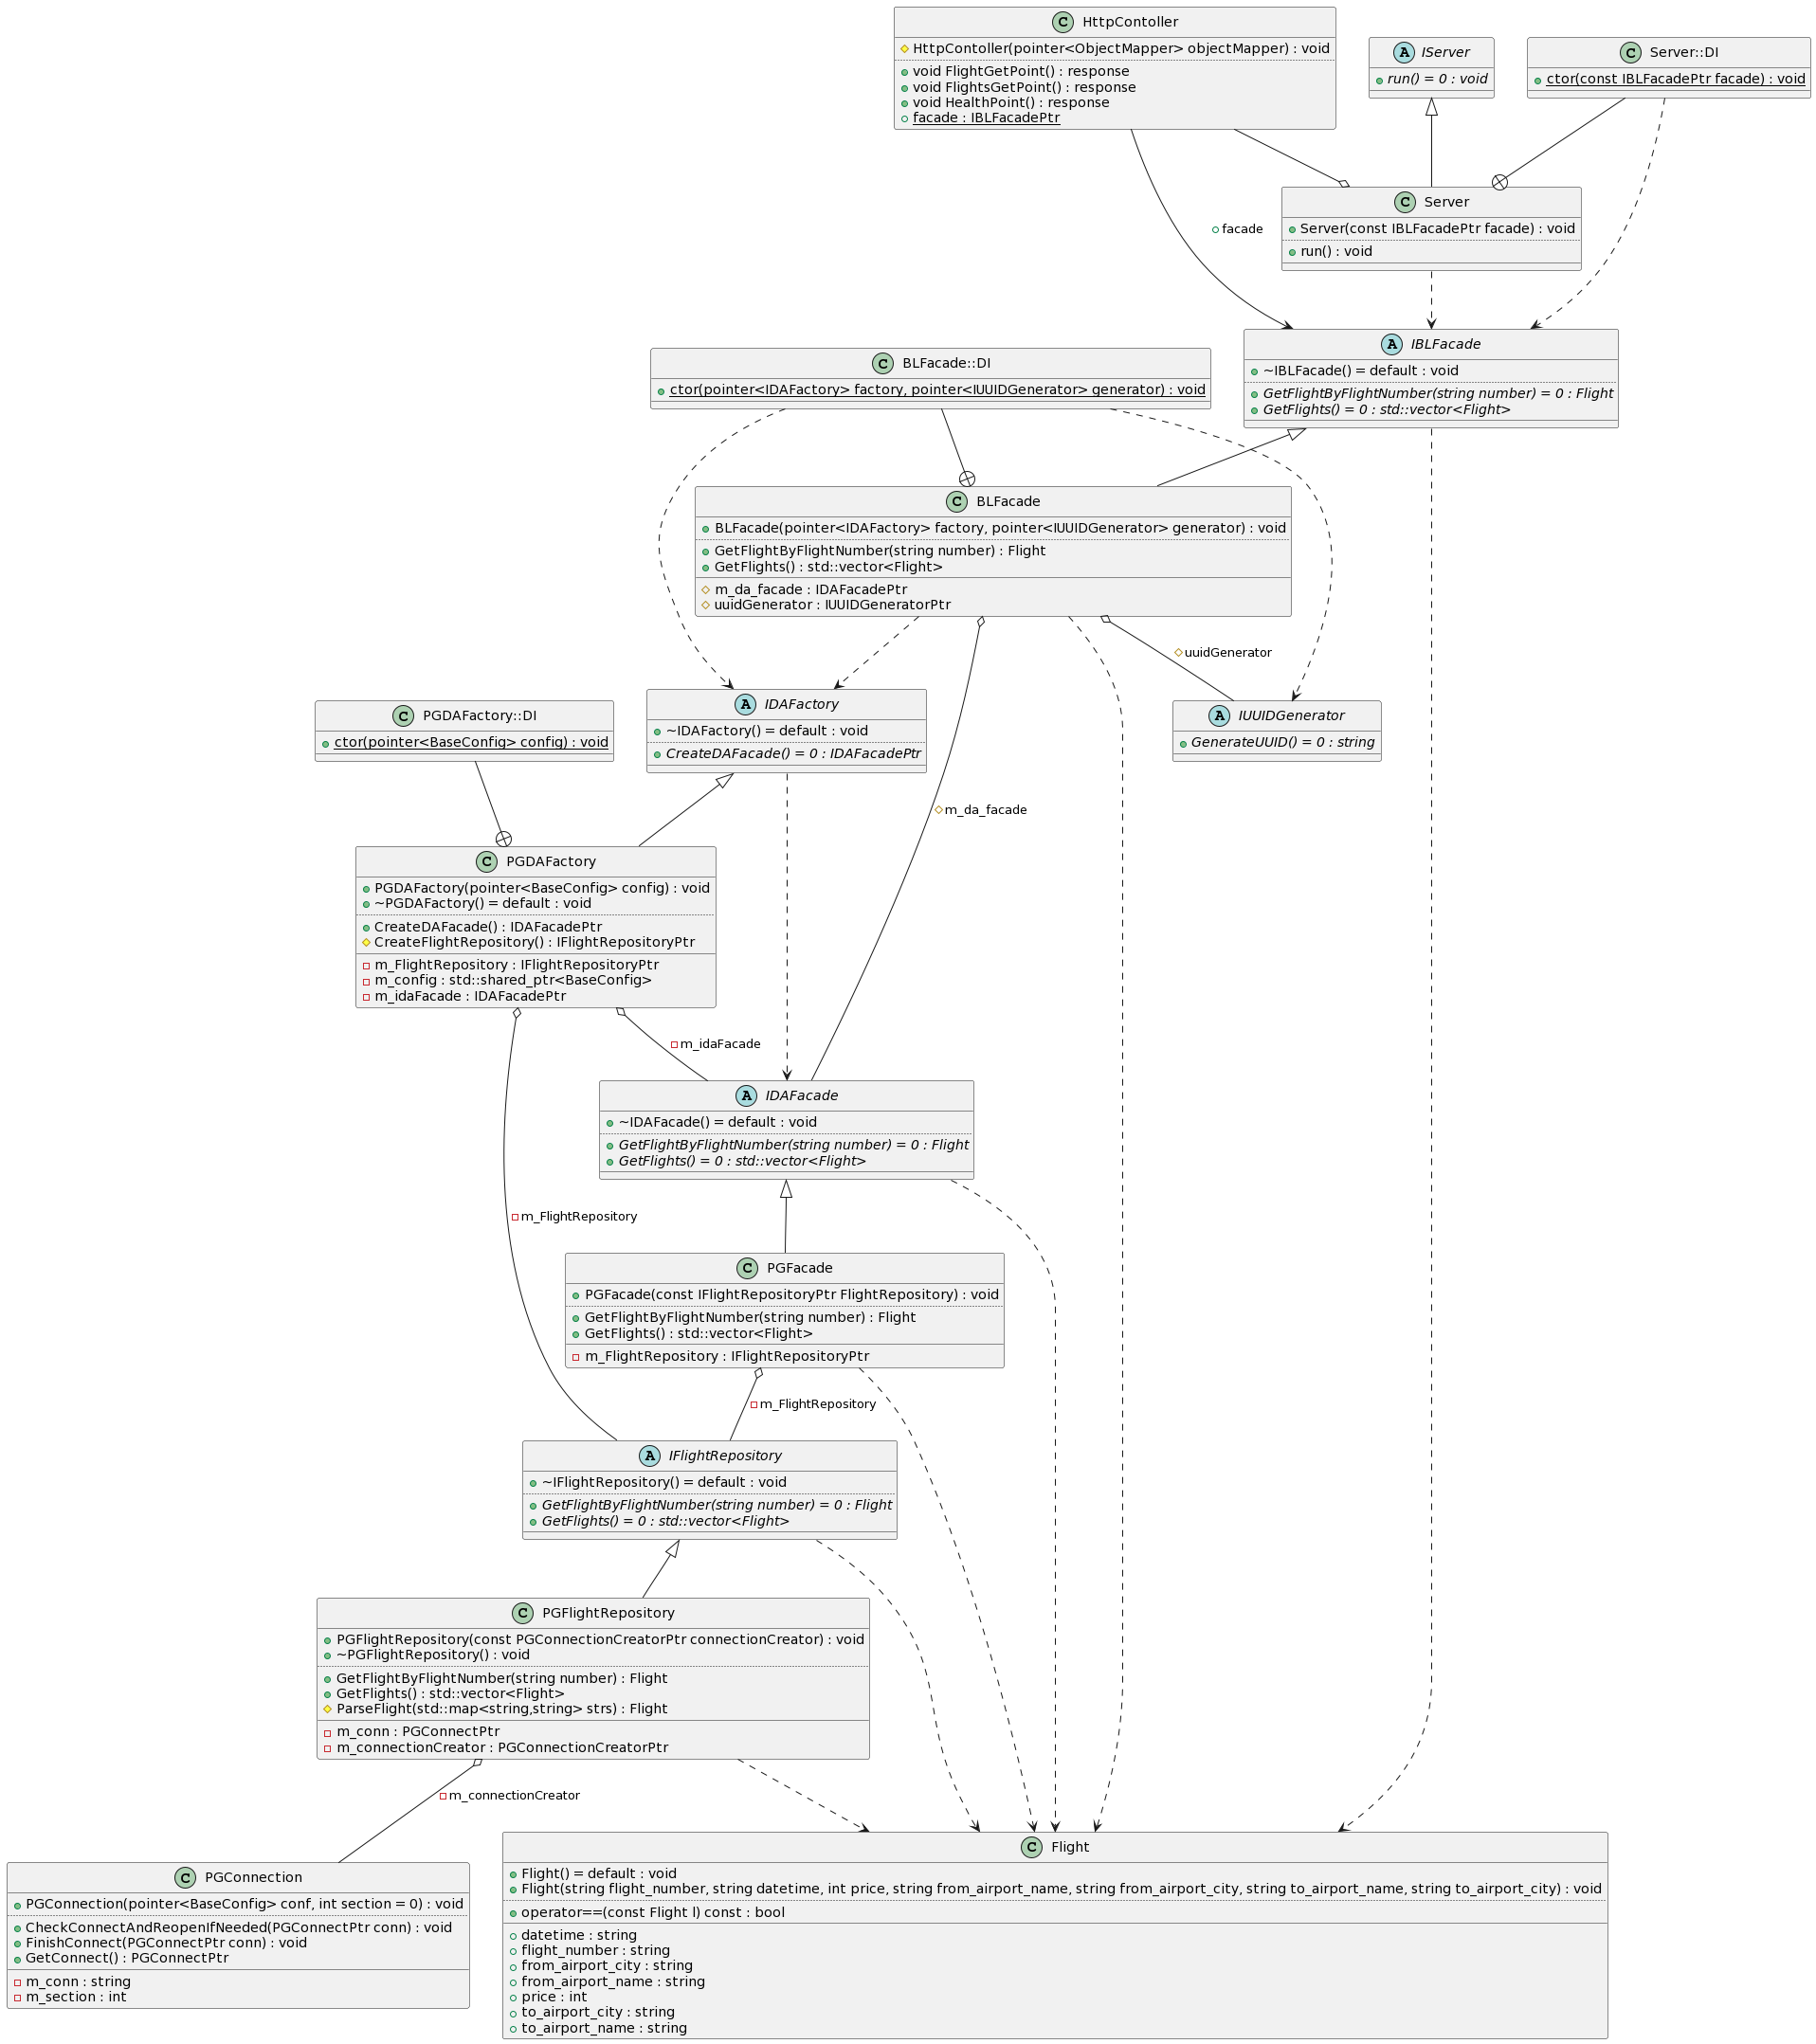
\includegraphics[width=1.05\textwidth]{../images/flights_uml.png}
    \caption{Диаграмма классов сервиса рейсов}
    \label{images:algorithm}
\end{figure}

\begin{figure}[H]
    \centering
    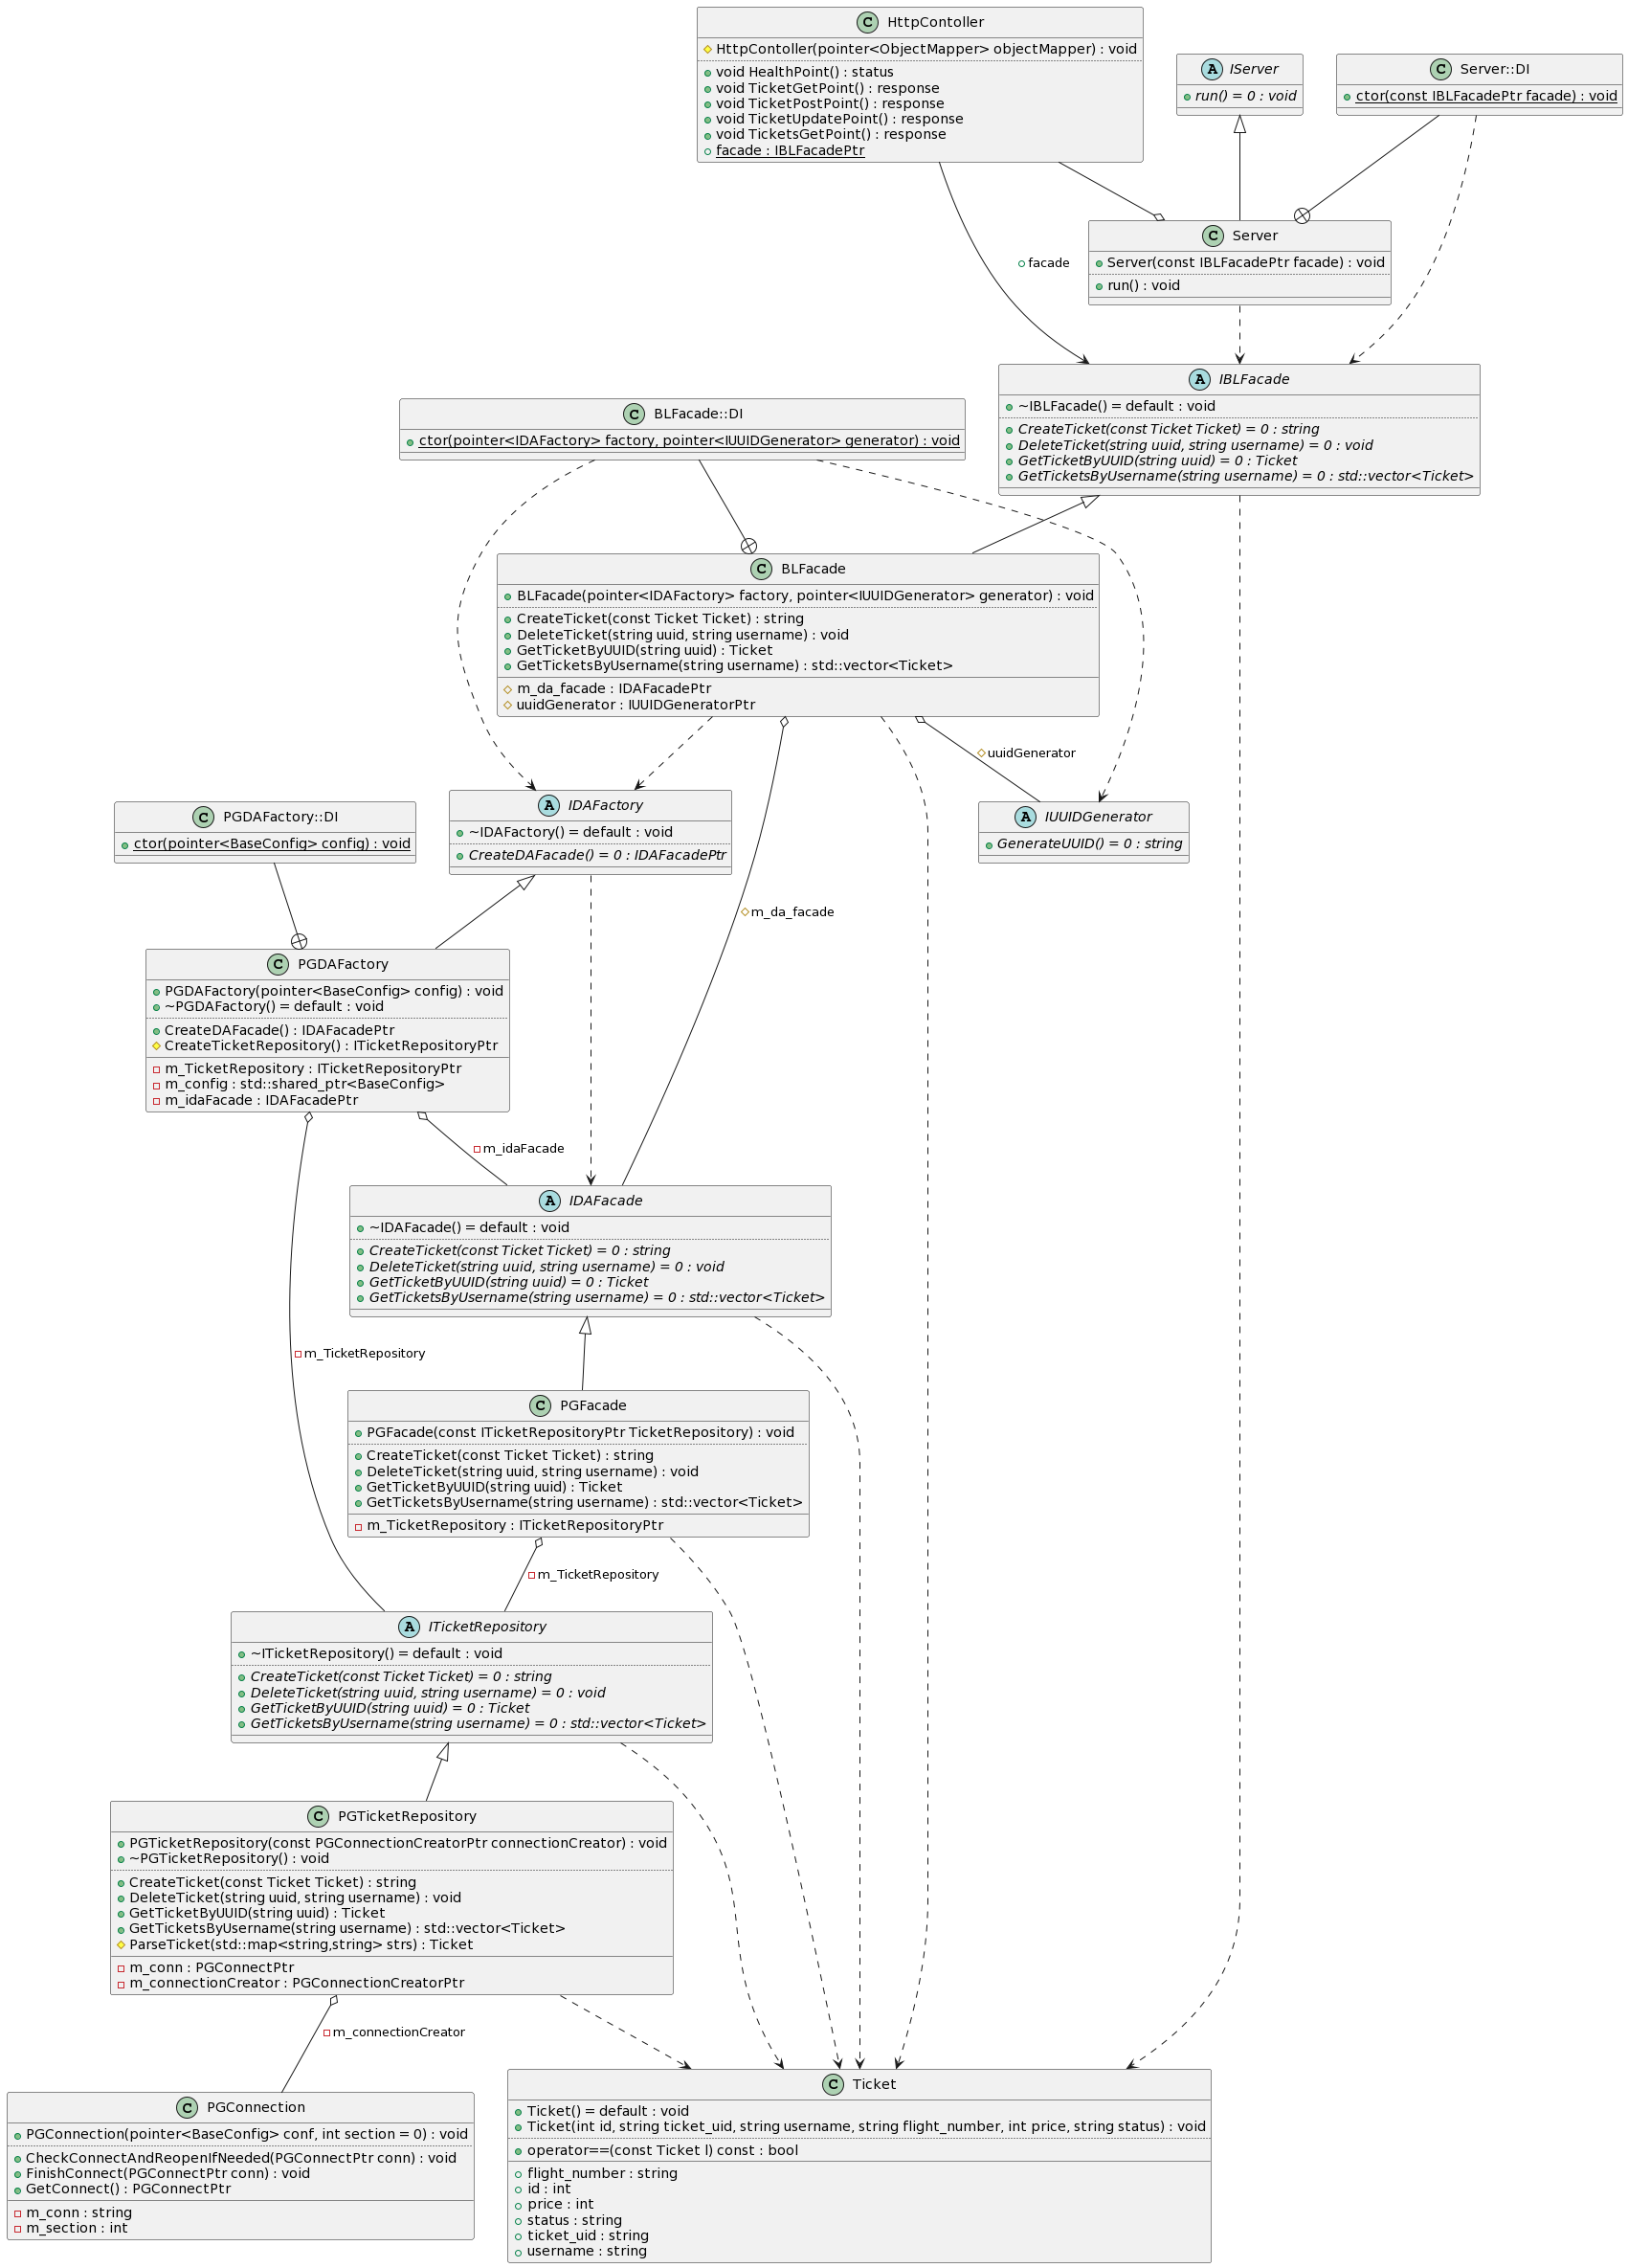
\includegraphics[width=1.05\textwidth]{../images/ticket_uml.png}
    \caption{Диаграмма классов сервиса билетов}
    \label{images:algorithm}
\end{figure}

\begin{figure}[H]
    \centering
    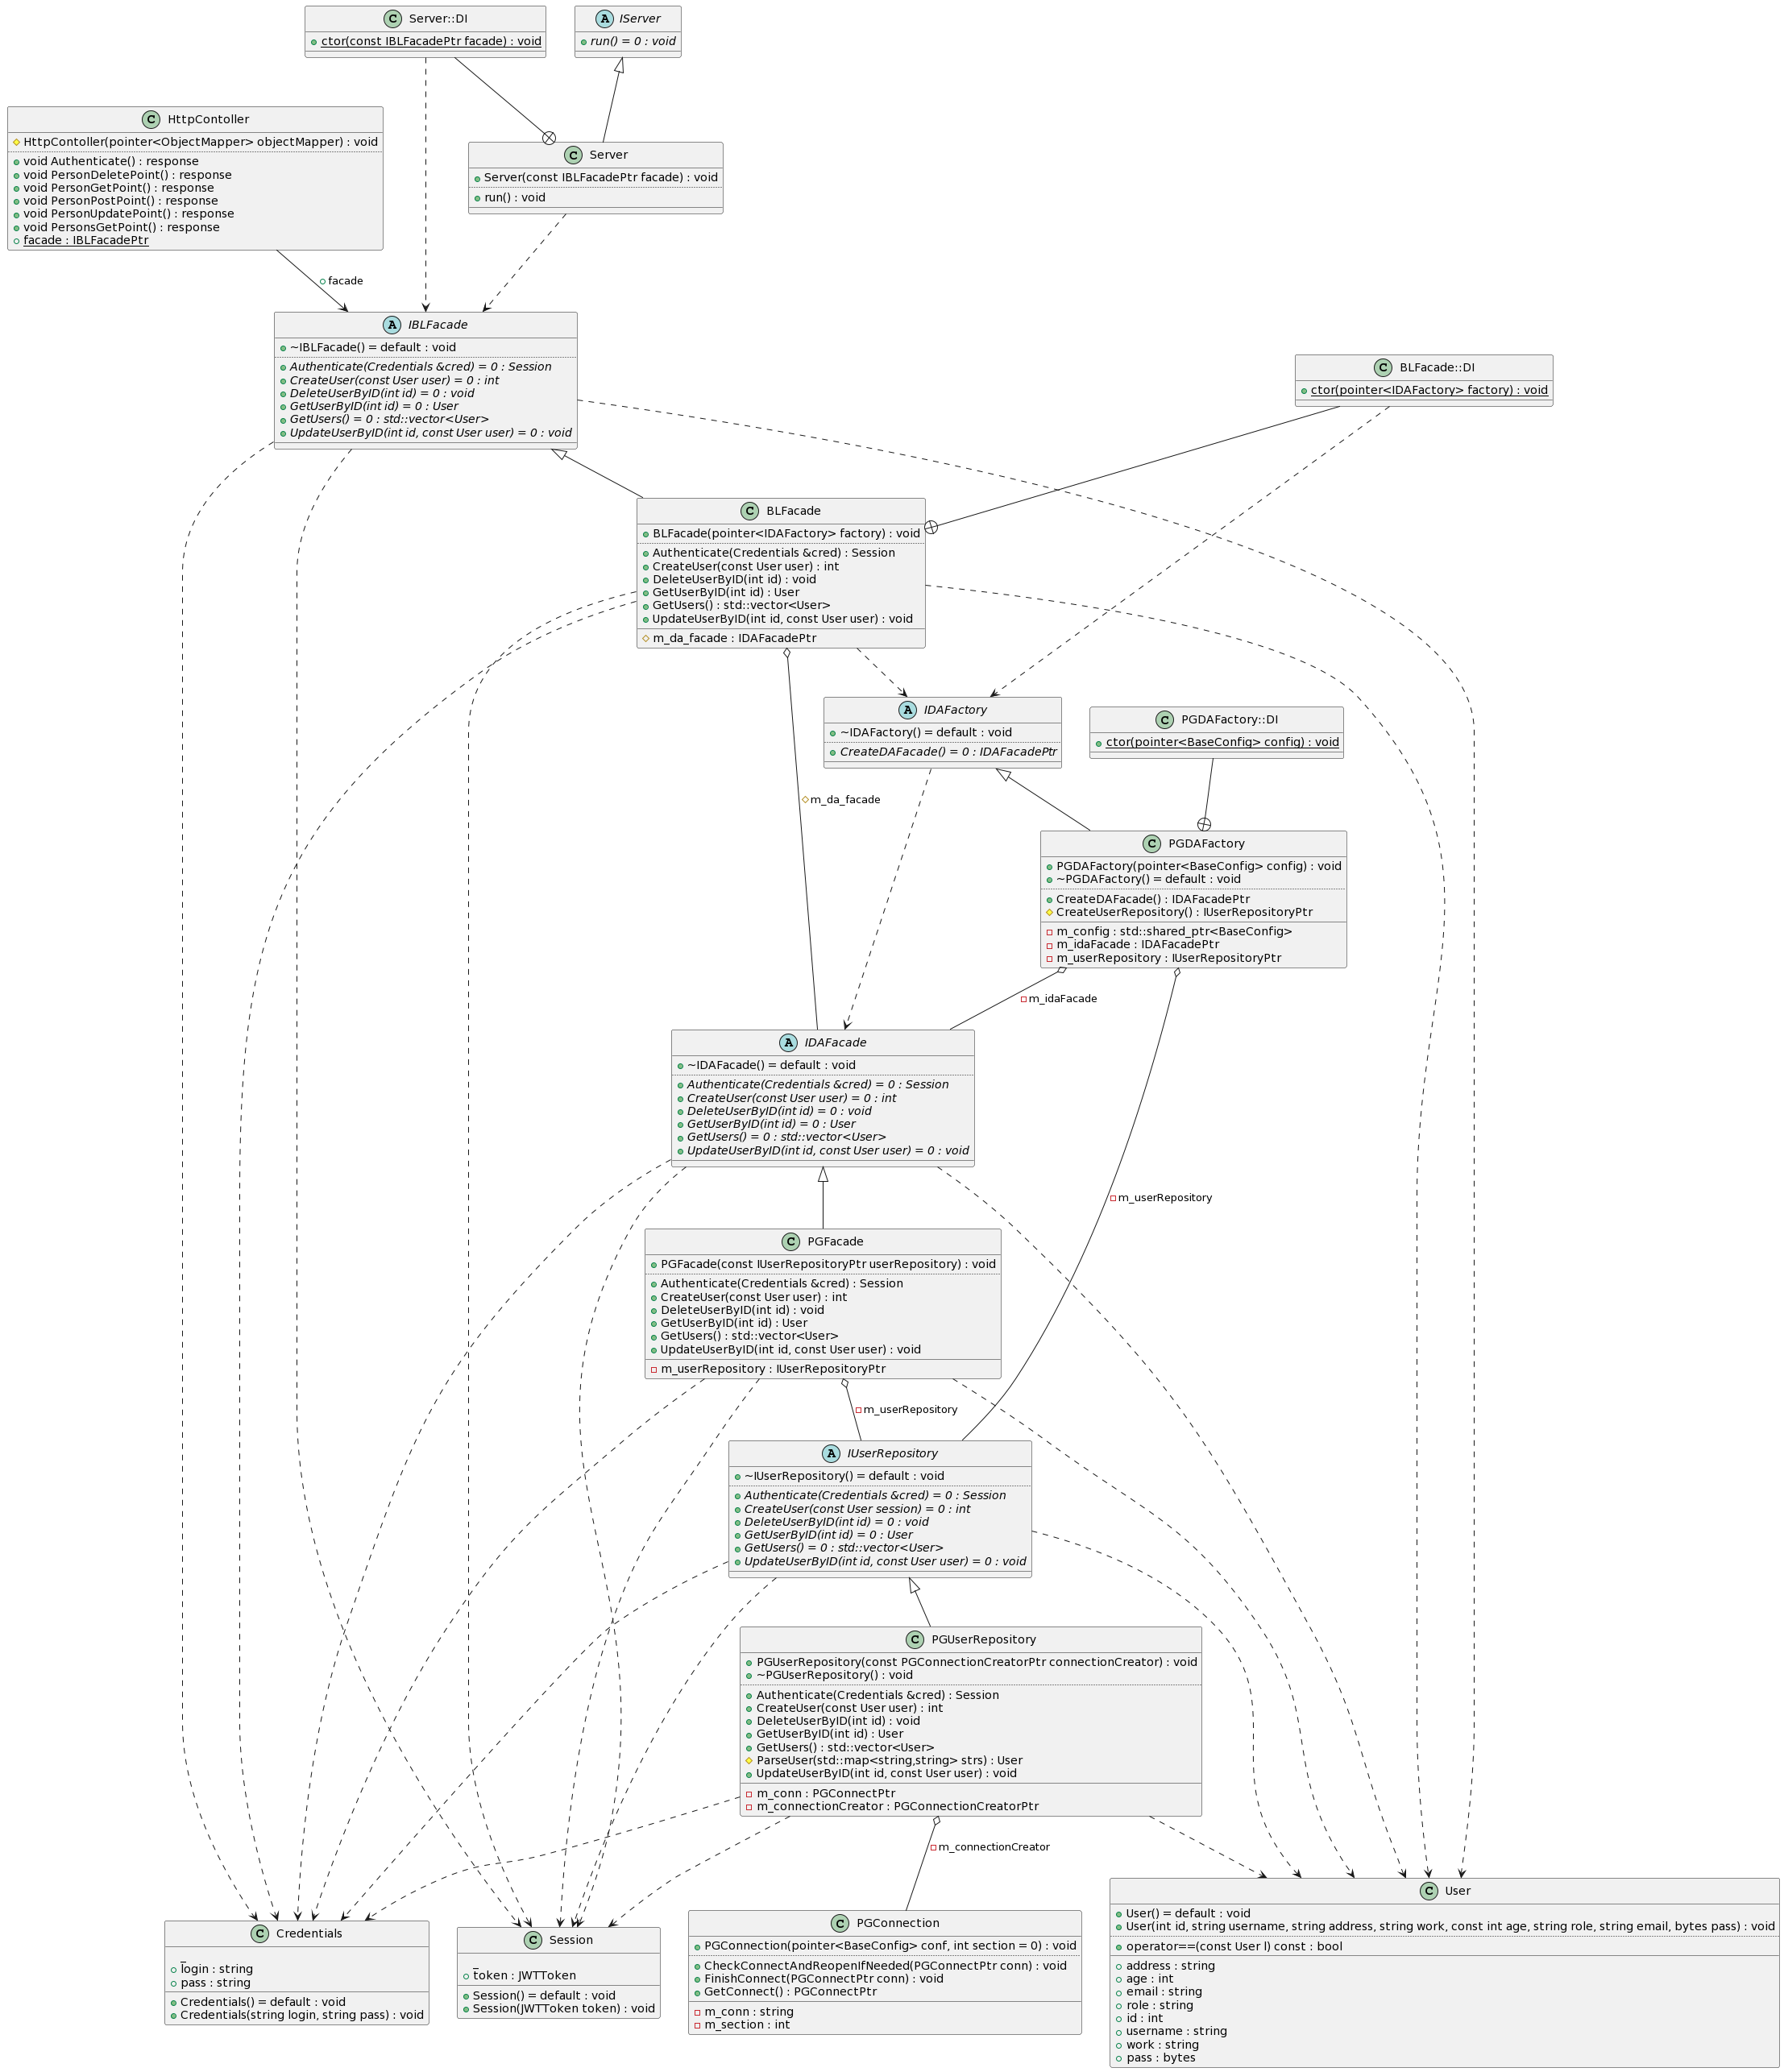
\includegraphics[width=1.05\textwidth]{../images/person_uml.png}
    \caption{Диаграмма классов сервиса сессий и пользователей}
    \label{images:algorithm}
\end{figure}

\begin{figure}[H]
    \centering
    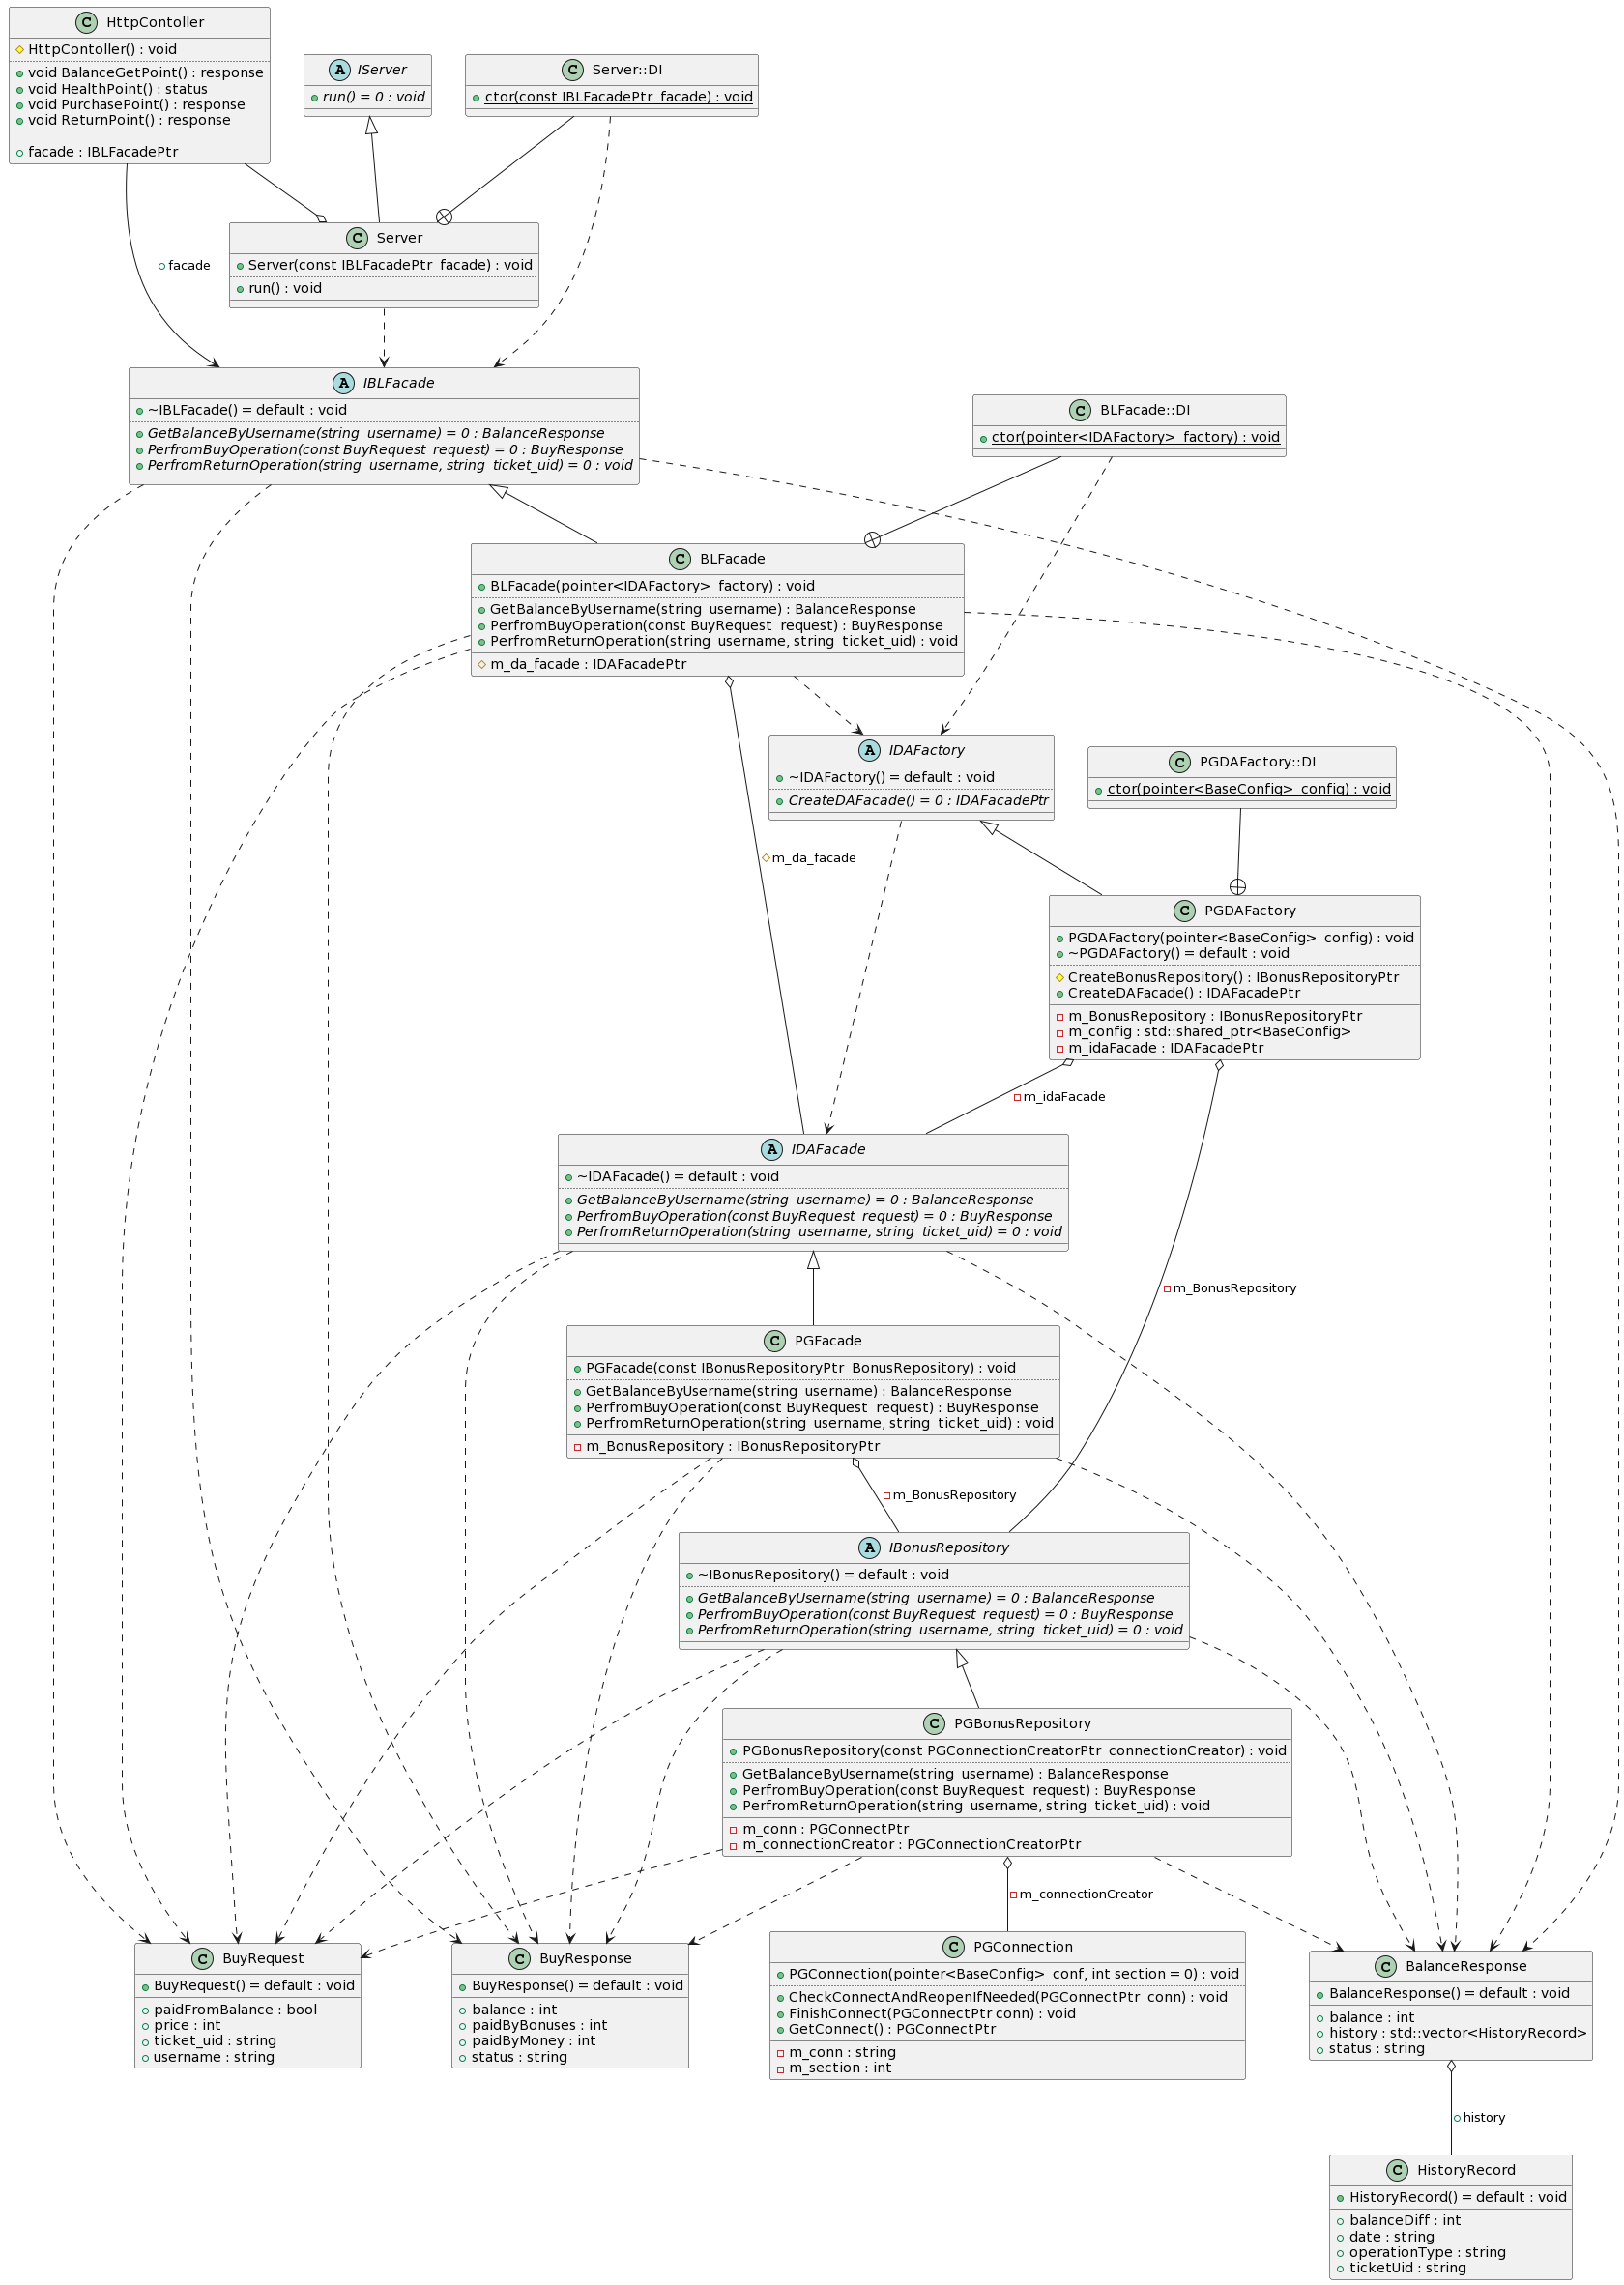
\includegraphics[width=1.05\textwidth]{../images/bonus_uml.png}
    \caption{Диаграмма классов сервиса программы лояльности}
    \label{images:algorithm}
\end{figure}

\begin{figure}[H]
    \centering
    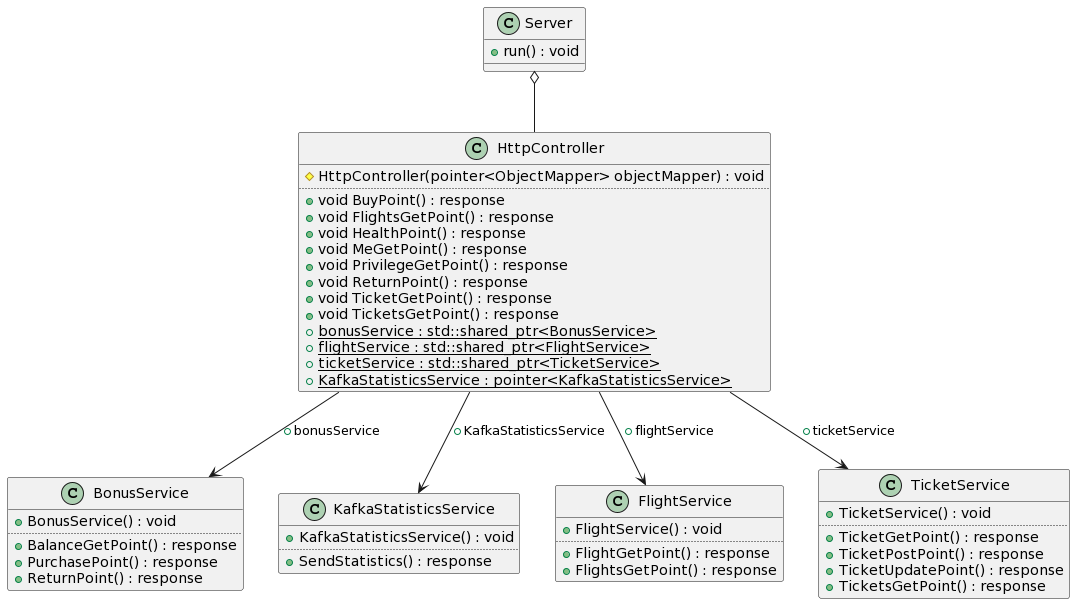
\includegraphics[width=1.05\textwidth]{../images/gateway_uml.png}
    \caption{Диаграмма классов сервиса-координатора}
    \label{images:algorithm}
\end{figure}

\begin{figure}[H]
    \centering
    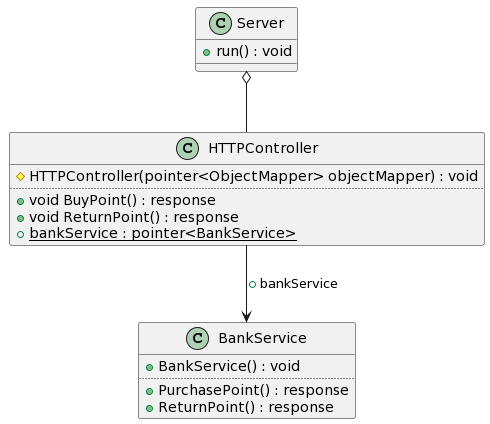
\includegraphics[width=1.05\textwidth]{../images/bank_uml.png}
    \caption{Диаграмма классов сервиса оплаты}
    \label{images:algorithm}
\end{figure}

\begin{figure}[H]
    \centering
    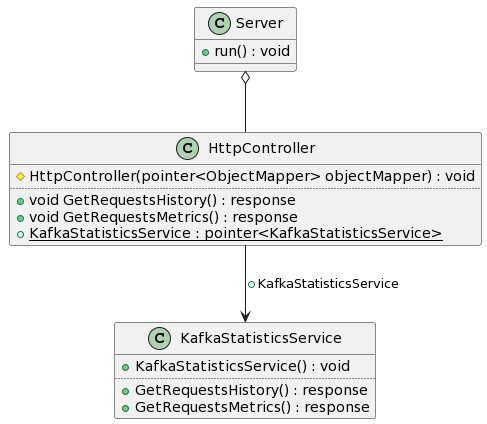
\includegraphics[width=1.05\textwidth]{../images/stat_uml.png}
    \caption{Диаграмма классов сервиса статистики}
    \label{images:algorithm}
\end{figure}


\newpage
\subsubsection{Описание классов сервисов}

Сервисы рейсов, билетов, программы лояльности и сессий и пользователей спроектированы похожим образом. Они имеют:
\begin{itemize}
    \item слой доступа к данным, реализованный с помощью паттерна <<Репозиторий>> для абстракции хранения, а также паттерна <<пул объектов>> для эффективного использования активных подключений к базе данных;
    \item слой логики работы сервиса;
    \item слой интерфейса -- слой связи с другими сервисами с помощью http-запросов.
\end{itemize}

Так как сервисы спроектированы одинаково, часть классов совпадают. Опишем их:
\begin{itemize}
    \item IDAFacade -- абстрактный интерфейс слоя доступа к данным; PGDAFacade -- реализация этого абстрактного интерфейса для работы с данными, хранящимися под управлением СУБД Postgres;
    \item IDAFactory -- абстрактный интерфейс фабрики объектов, относящихся к библиотеке работы с данными (интерфейс спроектирован в соответствии с паттерном <<фабрика объектов>>); PGDAFactory -- реализация этого абстрактного интерфейса для работы с данными, хранящимися под управлением СУБД Postgres;
    \item PGConnection -- пул активных подлключений к базе данных, спроектированный в соответствии с паттерном <<пул объектов>>;
    \item IBLFacade -- абстрактный интерфейс слоя логики; BLFacade -- реализация этого абстрактного интерфейса;
    \item IServer -- абстрактный интерфейс серверного приложения, предоставляющего интерфейс, описанный HTTPController; Server -- реализация этого интерфейса.
    \item HTTPController -- класс, описывающий набор  HTTP-методов, которые доступны на сервисе. Фактически занимается распаковкой данных, пришедших по сети, заполнением необходимых структур этими данными и вызовом функций, реализующих логику работы методов. Также занимается подготовкой результирующих данных к отправке по сети после выполнения запроса. 
\end{itemize}

Кроме того, каждый сервис имеет собственные классы. Опишем их.

\subsubsection{Описание классов сервиса рейсов}

\begin{itemize}
    \item Flight -- класс, описывающий рейс, имеет поля:
    \begin{itemize}
        \item datetime : string - дата и время рейса;
        \item price : int - цена рейса;
        \item flight\_number : int - номер рейса;
        \item from\_airport\_name/to\_airport\_name : string - аэропорты вылета и прилёта;
        \item from\_airport\_city/to\_airport\_city : string - города вылета и прилёта.
    \end{itemize}
    \item IFlightRepository -- абстрактный интерфейс для работы с данными рейсов (интерфейс спроектирован в соответствии с паттерном <<репозиторий>>). PGFlightRepository -- реализация этого абстрактного интерфейса для работы с данными, хранящимися под управлением СУБД Postgres.
\end{itemize}

\subsubsection{Описание классов сервиса билетов}

\begin{itemize}
    \item Ticket -- класс, описывающий билет, имеет поля:
    \begin{itemize}

        \item id : int - номер билета;
        \item price : int - цена билета;
        \item flight\_number : string - номер рейса;
        \item status : bool - статус (оплачен или отменён);
        \item ticket\_uid : string - идентификатор билета;
        \item username : string - владелец билета.
    \end{itemize}
    \item ITicketRepository -- абстрактный интерфейс для работы с данными билетов (интерфейс спроектирован в соответствии с паттерном <<репозиторий>>). PGTicketRepository -- реализация этого абстрактного интерфейса для работы с данными, хранящимися под управлением СУБД Postgres.
\end{itemize}

\subsubsection{Описание классов сервиса сессий и пользователей}

\begin{itemize}
    \item User -- класс, описывающий пользователя, имеет поля:
    \begin{itemize}
        \item id : int - идентификатор пользователя;
        \item login : string - логин пользователя;
        \item role : string - роль пользователя;
        \item age : int - возраст пользователя;
        \item mobilePhone : string - номер телефона
        \item email : string - почта
        \item password : string - пароль пользователя (в виде хэша).
    \end{itemize}
    \item Session -- класс, описывающий сессию пользователя, является JWT-token-ом;
    \item Credentials -- класс, который хранит логин и пароль пользователя.
    \item IUserRepository -- абстрактный интерфейс для работы с данными пользователей и сессий (интерфейс спроектирован в соответствии с паттерном <<репозиторий>>). PGUserRepository -- реализация этого абстрактного интерфейса для работы с данными, хранящимися под управлением СУБД Postgres.
\end{itemize}

\begin{itemize}
    \item BuyRequest -- класс, описывающий запрос на покупку билета, имеет поля:
    \begin{itemize}
        \item решение пользователя о списании или о начислении бонусов;
        \item цена билета;
        \item номер билета;
        \item имя пользователя.
    \end{itemize}
    \item BuyResponse -- класс, описывающий ответ на покупку билета, имеет поля:
    \begin{itemize}
        \item баланс счёта программы лояльности после покупки билета;
        \item количество денег, списанное за счёт бонусов;
        \item количество денег, списанное за счёт средств пользователя;
        \item статус счёта лояльности (золотой, серебряный, бронзовый) после покупки.
    \end{itemize}
    \item BalanceResponse -- класс, описывающий ответ на запрос информации о бонусном счёта и истории операций бонусного счёта, имеет поля:
    \begin{itemize}
        \item баланс счёта программы лояльности;
        \item статус счёта лояльности (золотой, серебряный, бронзовый);
        \item история операций (каждая запись содержит: абсолютное значение изменения баланса, дату операции, типа операции -- списание или начисление, идентификатор билета).
    \end{itemize}
    \item IBonusRepository -- абстрактный интерфейс для работы с данными программы лояльности (интерфейс спроектирован в соответствии с паттерном <<репозиторий>>). PGBonusRepository -- реализация этого абстрактного интерфейса для работы с данными, хранящимися под управлением СУБД Postgres.
\end{itemize}

\subsubsection{Описание классов сервиса-координатора}

\begin{itemize}
    \item HTTPController -- класс, описывающий набор  HTTP-методов, которые доступны на сервисе. Фактически предасвляет собой весь программный интерфейс системы. В своей работе для обслуживания приходящих запросов сервис использует интерфейсы сервисов программы лояльности (BonusService), рейсов (FlightService) и билетов (TicketService). Кроме того, сервис перенаправляет статистику запросов в очередь Kafka с помощью интерфейса KafkaStatistcsService.
    \item Server -- реализация серверного приложения, предоставляющего интерфейс, описанный HTTPController.
\end{itemize}

\subsubsection{Описание классов сервиса оплаты}

\begin{itemize}
    \item HTTPController -- класс, описывающий набор  HTTP-методов, которые доступны на сервисе (покупка и возврат билетов). В своей работе для обслуживания приходящих запросов сервис использует сервисы банка для выполнения транзакций со счётом пользователя.
    \item Server -- реализация серверного приложения, предоставляющего интерфейс, описанный HTTPController.
\end{itemize}

\subsubsection{Описание классов сервиса статистики}
\begin{itemize}
    \item HTTPController -- класс, описывающий набор  HTTP-методов, которые доступны на сервисе (просмотр истории запросов к системе и метрики, рассчитанные на основе этой истории). В своей работе для обслуживания приходящих запросов сервис использует очередь Kafka.
    \item Server -- реализация серверного приложения, предоставляющего интерфейс, описанный HTTPController.
\end{itemize}

\subsection*{Диаграмма действий}
\addcontentsline{toc}{subsection}{Диаграмма действий}

\begin{figure}[H]
    \centering
    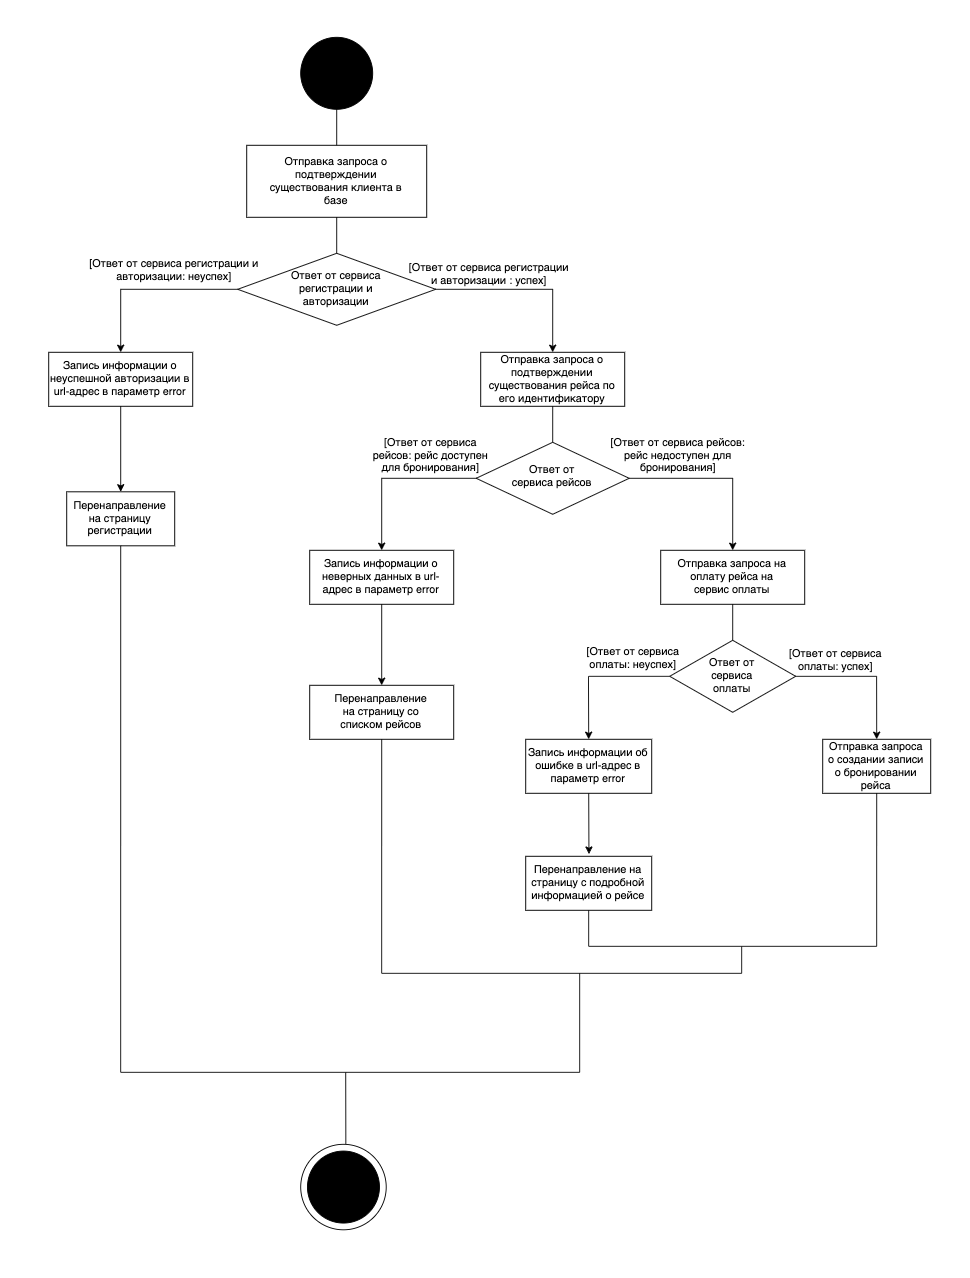
\includegraphics[width=1.05\textwidth]{../images/algorithm.jpg}
    \caption{Страница со статистикой}
    \label{images:algorithm}
\end{figure}



\subsection*{Диаграмма последовательности действий}
\addcontentsline{toc}{subsection}{Диаграмма последовательности действий}

Диаграмма последовательности действий представлена на рисунке 14.

\begin{figure}[H]
    \centering
    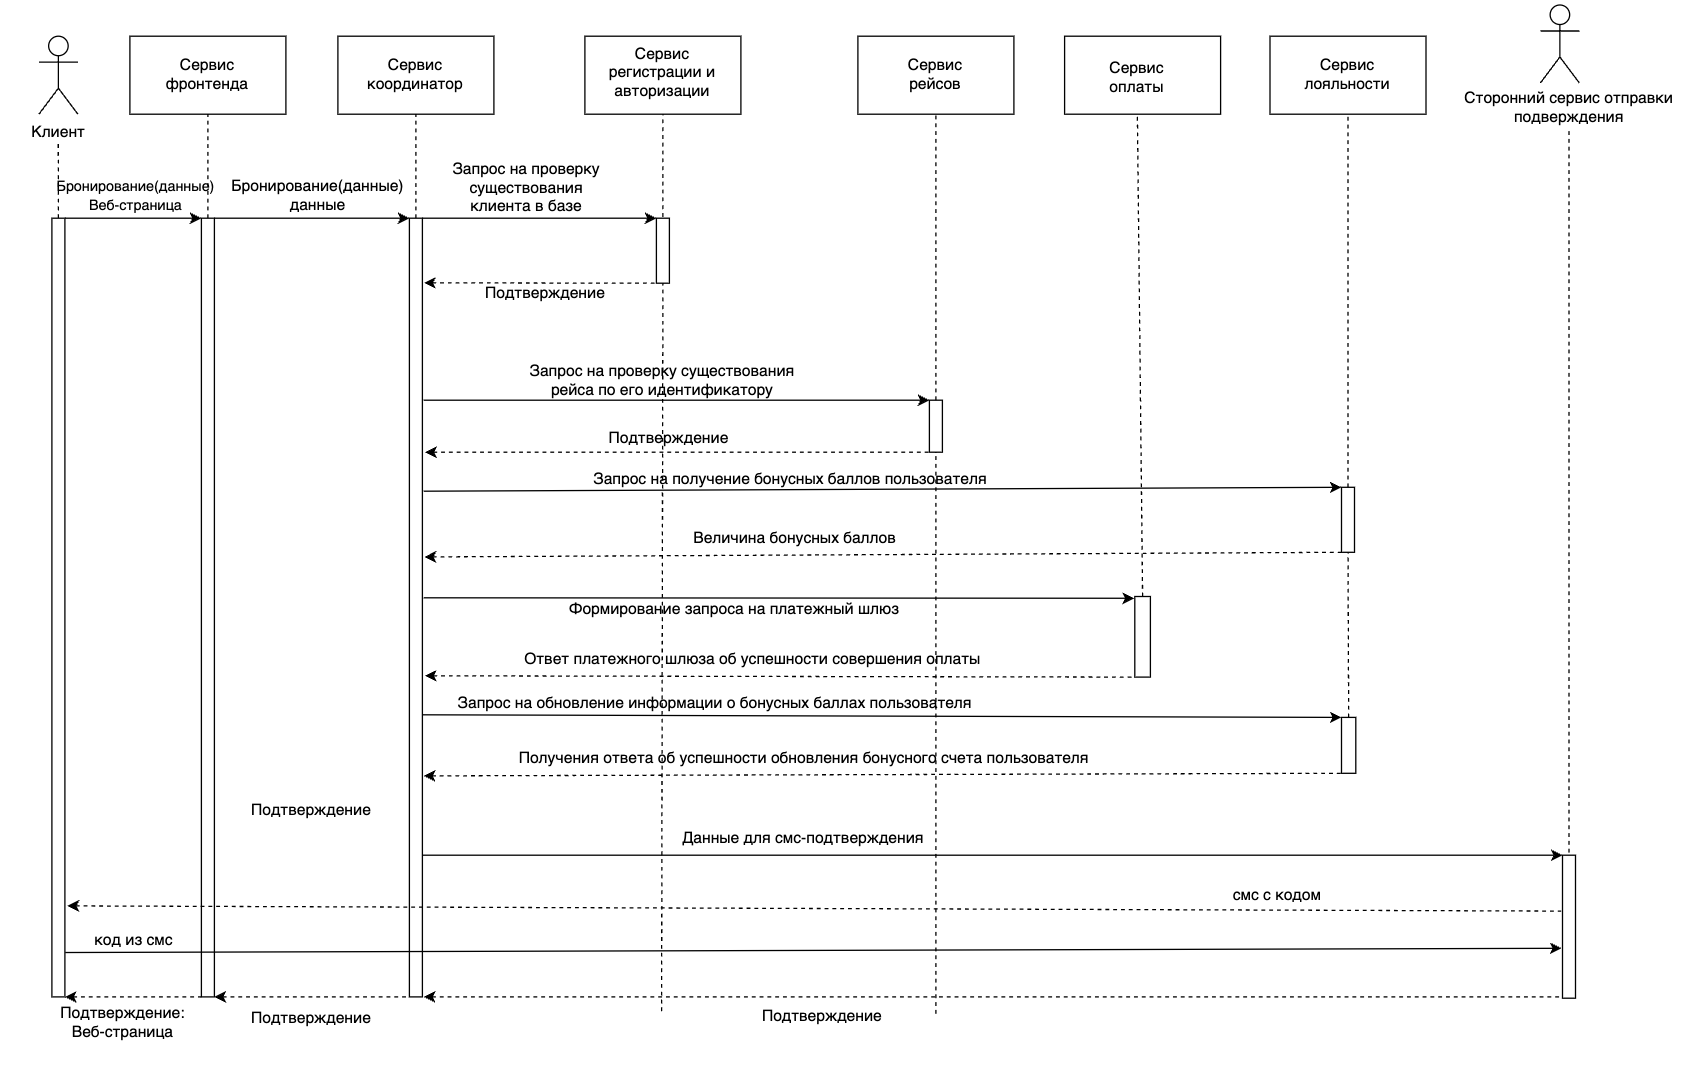
\includegraphics[width=1.05\textwidth]{../images/diagramm_1.jpg}
    \caption{Диаграмма последовательности действий}
    \label{images:algorithm}
\end{figure}


\subsection*{Диаграмма потоков данных}
\addcontentsline{toc}{subsection}{Диаграмма потоков данных}

Рассматриваемая система предполагает распределенное хранение данных.
Диаграмма потоков данных, представленная на рисунке 15, позволяет описать распределение сохраняемой информации в хранилищах данных.

\begin{figure}[H]
    \centering
    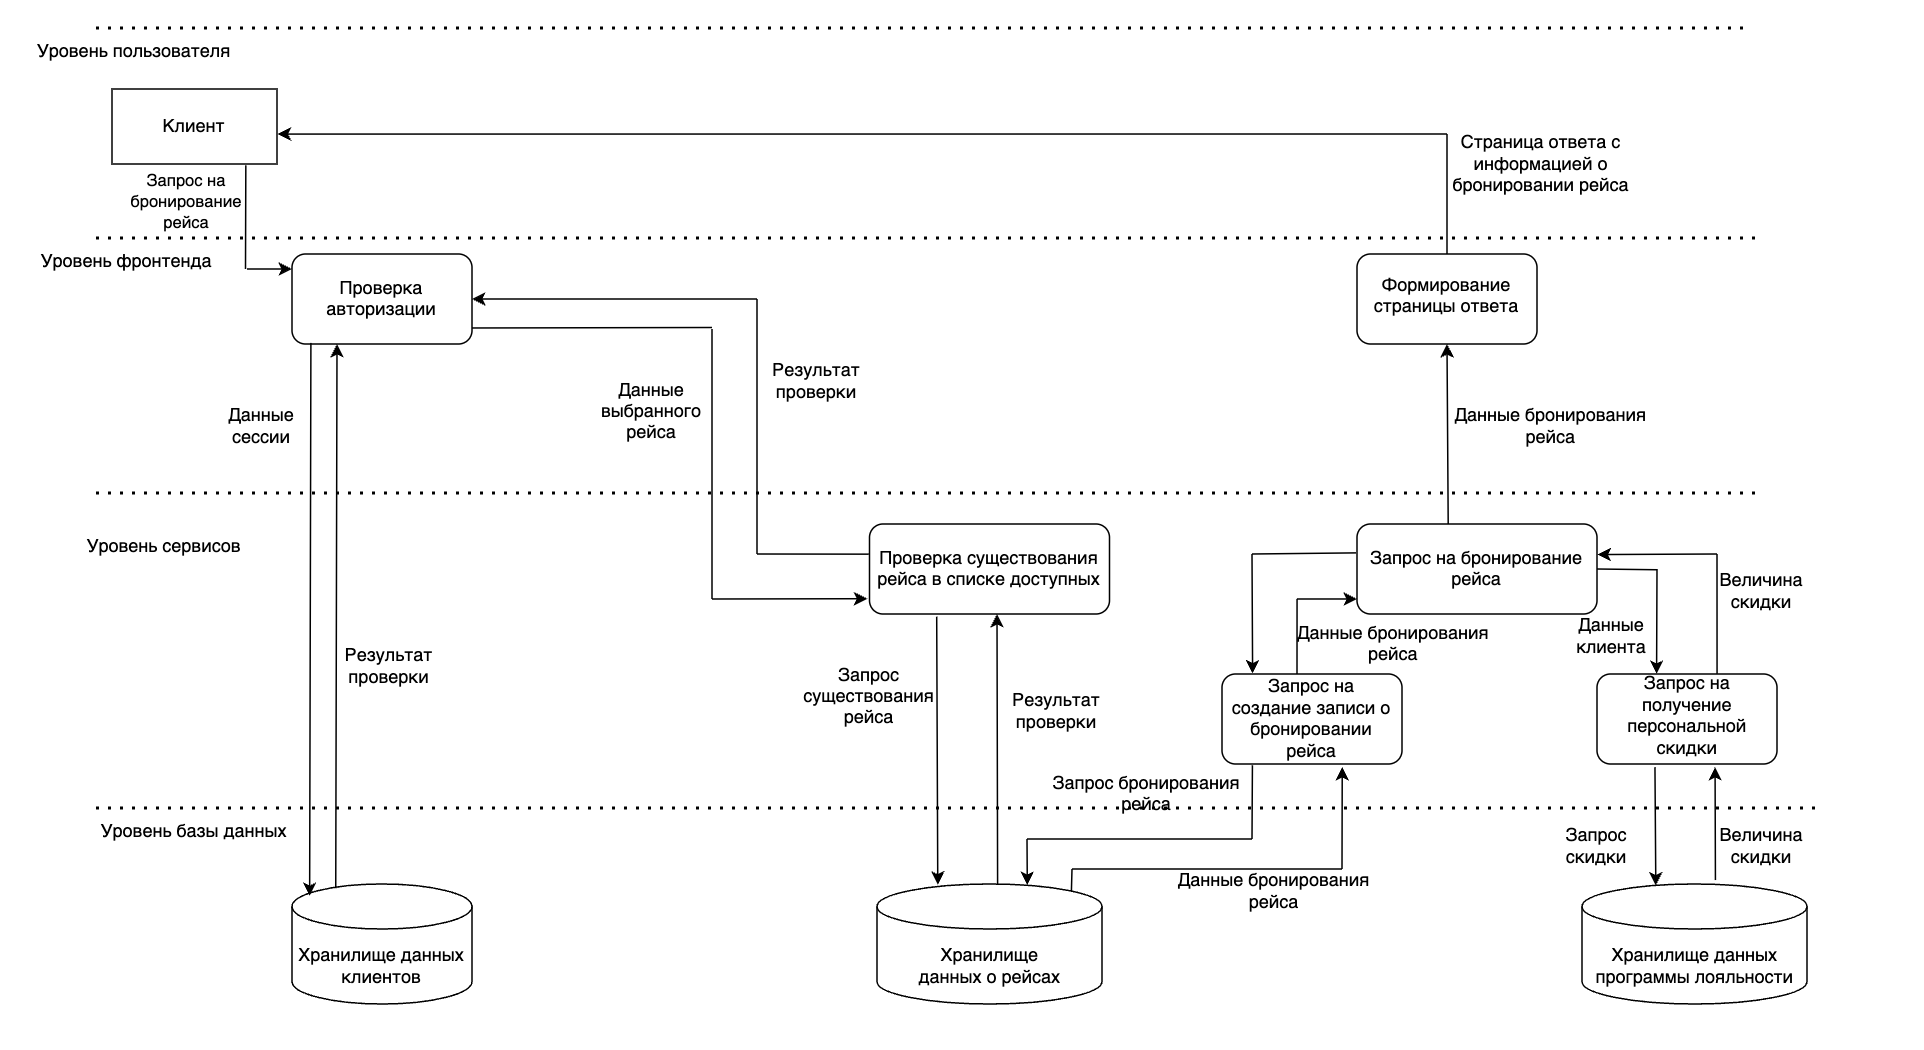
\includegraphics[width=1.05\textwidth]{../images/diagramm_2.jpg}
    \caption{Диаграмма потоков данных}
    \label{images:algorithm}
\end{figure}


\newpage
\section*{Высокоуровневый дизайн пользовательского интерфейса}
\addcontentsline{toc}{section}{Высокоуровневый дизайн пользовательского интерфейса}

Пользовательский интерфейс в разрабатываемой системе представляет собой web-интерфейс, доступ к которому осуществляется через браузер (тонкий клиент). 
Страница системы состоит из <<шапки>>, бокового меню и основной части.  

Обобщенно структуру страниц системы можно представить следующим образом:
\begin{itemize}
  \item страница авторизации;
	\item страница регистрации;
	\item страница со списком полетов;
	\item страница со списком купленных и сданных билетах;
	\item страница с информацией о пользователе и историей покупок билетов;
	\item страница со статистикой сервиса-координатора.
\end{itemize}

Данные страницы представленны на рисунках    приведены примеры описанных страниц.

\begin{figure}[H]
    \centering
    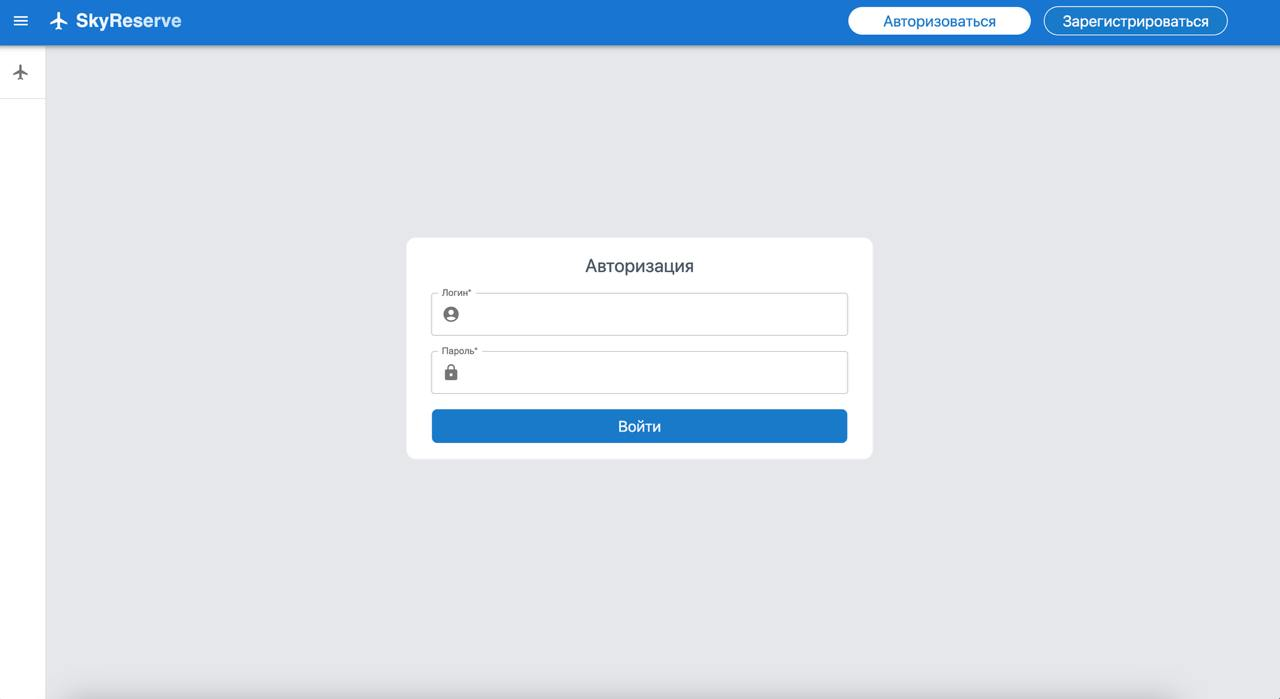
\includegraphics[width=1.05\textwidth]{../images/authorization_mpi.jpg}
    \caption{Страница авторизации}
    \label{images:algorithm}
\end{figure}

\begin{figure}[H]
    \centering
    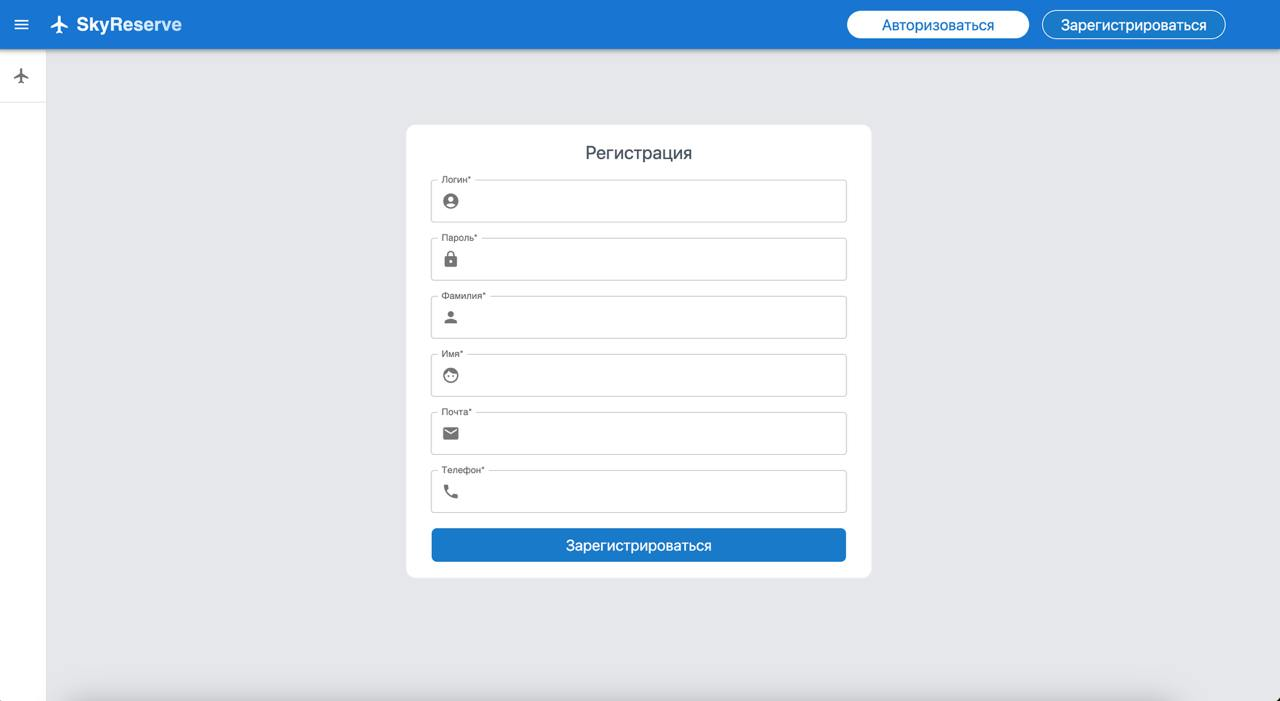
\includegraphics[width=1.05\textwidth]{../images/registration_mpi.jpg}
    \caption{Страница регистрации}
    \label{images:algorithm}
\end{figure}

\begin{figure}[H]
    \centering
    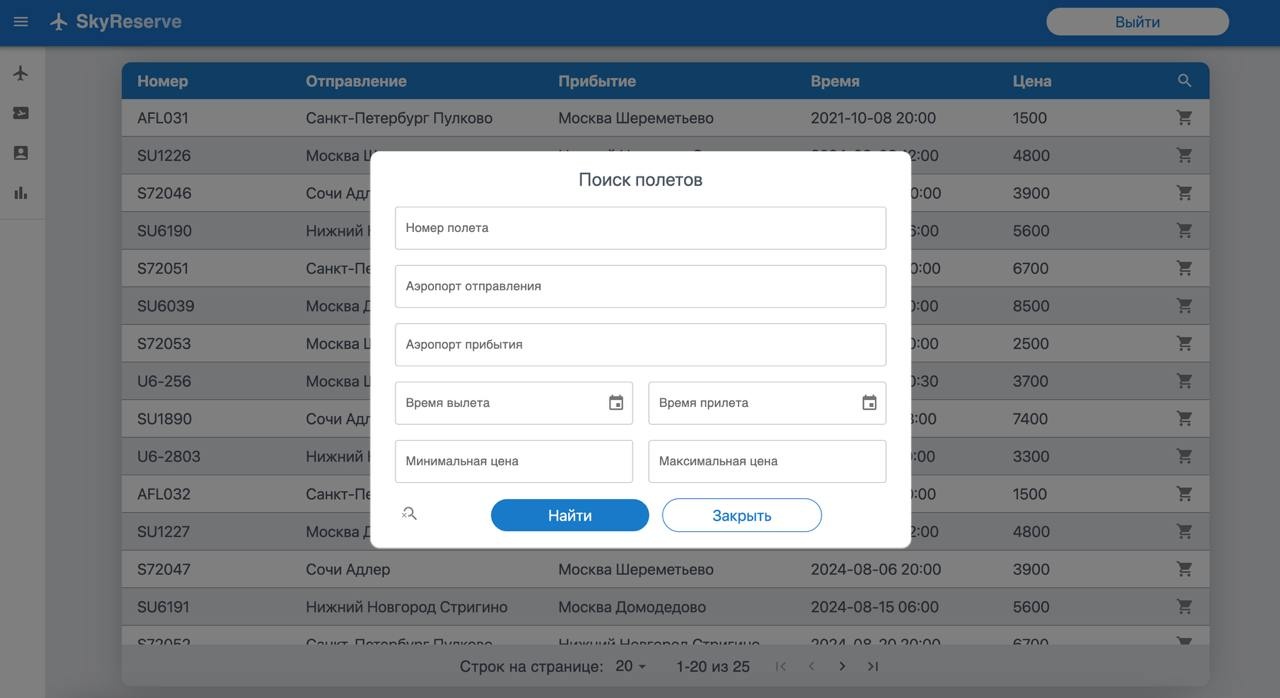
\includegraphics[width=1.05\textwidth]{../images/reserve_mpi.jpg}
    \caption{Страница с полетами}
    \label{images:algorithm}
\end{figure}

\begin{figure}[H]
    \centering
    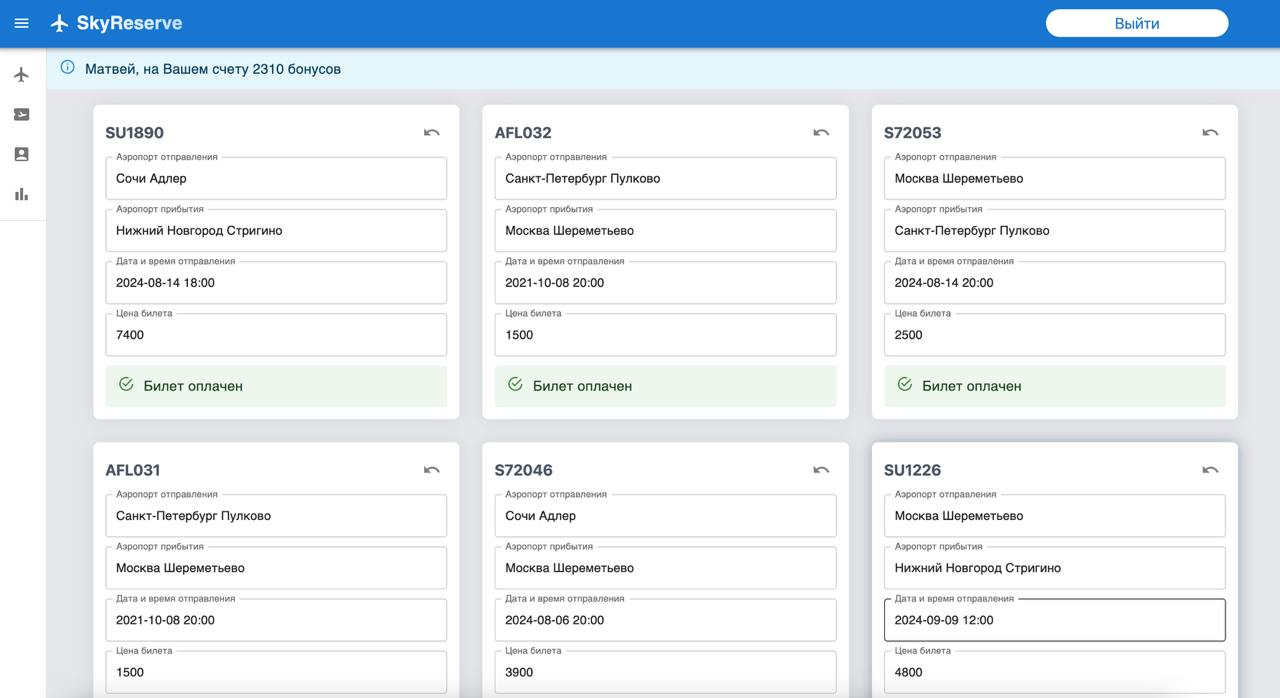
\includegraphics[width=1.05\textwidth]{../images/reservations_mpi.jpg}
    \caption{Страница с купленными и сданными билетами}
    \label{images:algorithm}
\end{figure}

\begin{figure}[H]
    \centering
    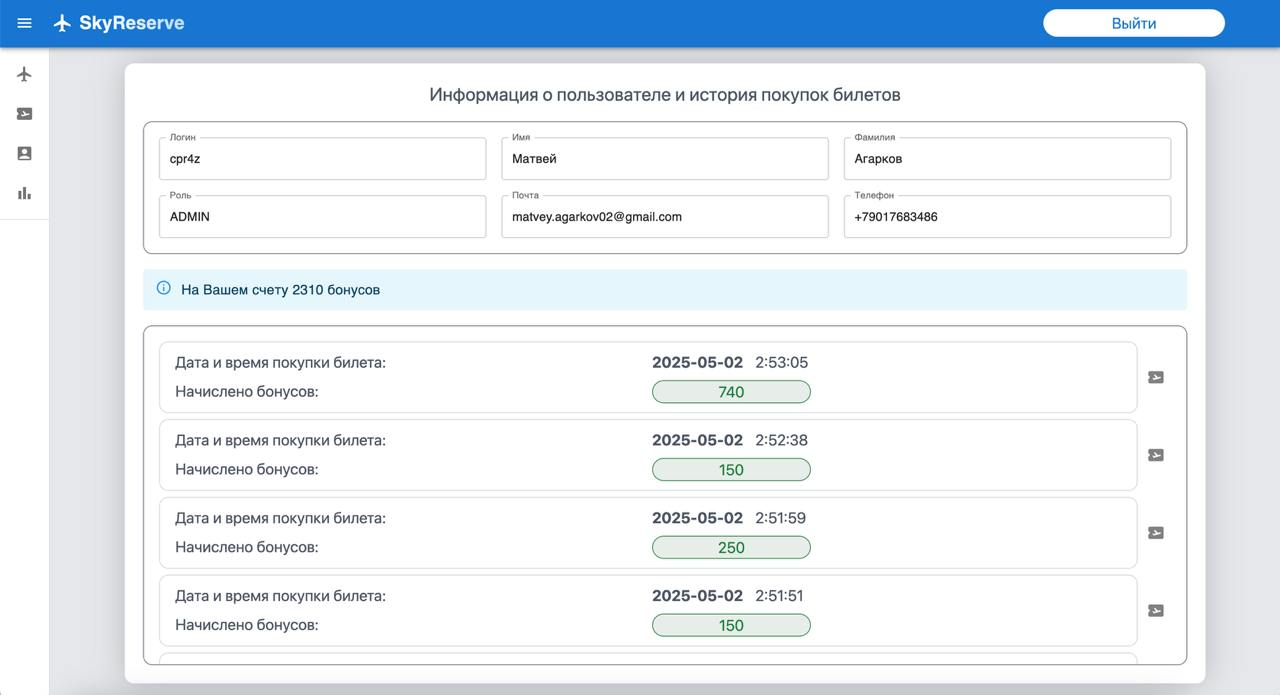
\includegraphics[width=1.05\textwidth]{../images/person_mpi.jpg}
    \caption{Страница с информацией о пользователе и историей покупок}
    \label{images:algorithm}
\end{figure}

\begin{figure}[H]
    \centering
    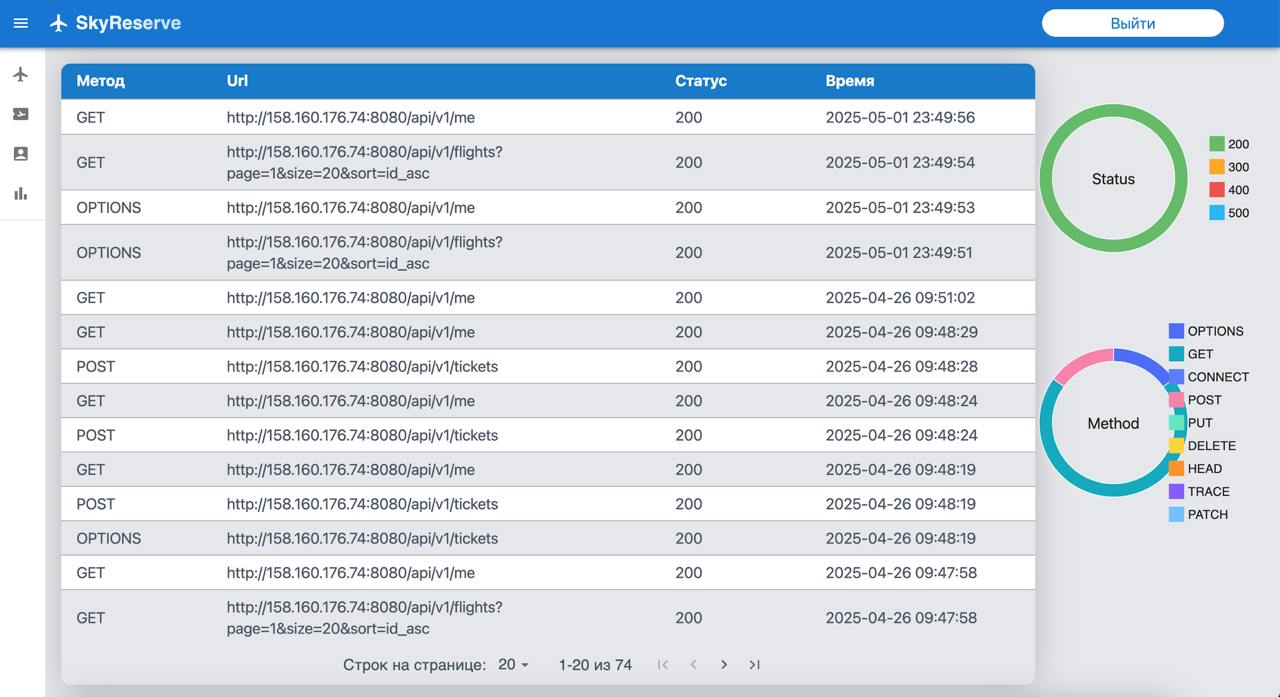
\includegraphics[width=1.05\textwidth]{../images/stat_mpi.jpg}
    \caption{Страница со статистикой}
    \label{images:algorithm}
\end{figure}


\section*{Физический дизайн}
\addcontentsline{toc}{section}{Физический дизайн}

\subsection*{Выбор системы развертывания компонентов распределенной системы}
\addcontentsline{toc}{subsection}{Выбор системы развертывания компонентов распределенной системы}

Согласно требованиям технического задания, разрабатываемая система должна быть распределенной. Характерной особенностью распределенных систем является высокое многообразие используемых технологий. Особенно непростая ситуация возникает, когда разные компоненты системы используют разные версии одной и той же библиотеки. Для того чтобы компоненты не конфликтовали друг с другом, необходимо ввести требование изолированности. В этом случае приходится использовать отдельные серверы, что может быть экономически нецелесообразно, либо использовать контейнеризацию. 

Контейнеризация -- это методология разработки и управления приложениями, которая позволяет упаковывать приложение и все его зависимости в изолированный контейнер (образ изолируемой части системы, содержащий приложение со всеми его зависимостям). Контейнеры обеспечивают среду выполнения для приложения, которая полностью отделена от других контейнеров и основной системы. Это облегчает развертывание, масштабирование и управление приложениями, а также обеспечивает надежность и безопасность при работе в различных средах. 

В качестве платформы для автоматизации развертывания, масштабирования и управления контейнеризированными приложениями на серверах было решено использовать Kubernetes. Такое решение было принято в результате следующего сравнительного анализа.

Существует несколько аналогов Kubernetes, которые также предоставляют возможности для управления контейнеризированными приложениями:
\begin{enumerate}
    \item Docker Swarm -- это оркестратор контейнеров, разработанный Docker, который позволяет управлять кластером Docker-хостов и запускать контейнеры в них. Он более прост в использовании по сравнению с Kubernetes, но может быть менее мощным в некоторых аспектах.
    \item Apache Mesos -- это распределенная система управления ресурсами, которая также поддерживает запуск контейнеров. Он предоставляет более общий подход к управлению ресурсами и приложениями, чем Kubernetes.
    \item Amazon ECS (Elastic Container Service) -- это управляемый сервис от Amazon Web Services для запуска и управления контейнерами на инфраструктуре AWS. Он предлагает простой способ запуска и масштабирования контейнеров без необходимости управления инфраструктурой.
\end{enumerate}

Достоинства Kubernetes по сравнению с аналогами:
\begin{itemize}
    \item Мощные возможности оркестрации: Kubernetes предоставляет широкий спектр возможностей для управления и автоматизации развертывания приложений в контейнерах.
    \item Большое сообщество и экосистема: Kubernetes имеет активное сообщество разработчиков и широкий выбор инструментов и плагинов для расширения его функциональности.
    \item Поддержка различных облачных и локальных сред: Kubernetes поддерживает различные облачные провайдеры и может быть развернут как локально, так и в облаке.
\end{itemize}

\subsection*{Выбор операционной системы}
\addcontentsline{toc}{subsection}{Выбор операционной системы}
Согласно требованиям технического задания, разрабатываемый портал должен обладать высокой доступностью, работать на типичных архитектурах ЭВМ (Intel x86, Intel x64), а так же быть экономически недорогим для сопровождения. Таким образом, можно сформулировать следующие требования к операционной системе:
\begin{itemize}
    \item Распространенность. На рынке труда должно быть много специалистов, способных администрировать распределенную систему, работающую под управлением выбранной операционной системы.
    \item Надежность. Операционная система должна широко использоваться в стабильных проектах, таких как Mail.Ru, Vk.com, Google.com. Эти компании обеспечивают высокую работоспособность своих сервисов, и на их опыт можно положиться.
    \item Наличие требуемого программного обеспечения. Выбор операционной системы недолжен ограничивать разработчиков в выборе программного обеспечения, библиотек.
    \item Цена.
\end{itemize}

Под данные требования лучше всего подходит ОС Ubuntu. Ubuntu -- это дистрибутив, использующий ядро Linux. Как и все дистрибутивы Linux, Ubuntu является ОС с открытым исходным кодом, бесплатным для использования. 

\subsection*{Выбор СУБД}
\addcontentsline{toc}{subsection}{Выбор СУБД}
В качестве СУБД была выбрана PostgreSQL, так как она наилучшим образом подходит под требования разрабатываемой системы:
\begin{itemize}
    \item Масштабируемость: PostgreSQL поддерживает горизонтальное масштабирование, что позволяет распределить данные и запросы между несколькими узлами базы данных. Это особенно полезно в географически распределенных системах, где данные и пользователи могут быть разбросаны по разным регионам.
    \item Географическая репликация: PostgreSQL предоставляет возможность настройки репликации данных между различными узлами базы данных, расположенными в разных географических зонах. Это позволяет обеспечить отказоустойчивость и более быстрый доступ к данным для пользователей из разных частей мира.
    \item Гибкость и функциональность: PostgreSQL обладает широким набором функций и возможностей, что делает его подходящим для различных типов приложений и использования в распределенной среде. Он поддерживает сложные запросы, транзакции, хранимые процедуры и многое другое.
    \item Надежность и отказоустойчивость: PostgreSQL известен своей надежностью и стабильностью работы. В распределенной географической системе это особенно важно, поскольку он способен обеспечить сохранность данных и доступность даже при сбоях в отдельных узлах.
\end{itemize}

\subsection*{Выбор языка разработки и фреймворков компонент портала}
Проанализируем техническое задание на разработку портала. Исходя из приведенных требований к системе, можно выявить требования к языку программирования:
\begin{itemize}
    \item Совместимость с выбранными ранее технологиями. Выбранный язык должен уметь взаимодействовать с ОС Linux, СУБД PostgreSQL.
    \item Производительность: C++ является компилируемым языком программирования, что позволяет создавать быстродействующие приложения. Он обладает низким уровнем абстракции, что позволяет разработчику более тонко управлять ресурсами и оптимизировать производительность программы.
    \item Расширяемость: C++ обладает возможностью использовать объектно-ориентированный подход к программированию, что делает его удобным для создания сложных и масштабируемых систем.
\end{itemize}

Выбор oatpp в качестве фреймворка для разработки программного обеспечения также имеет свои преимущества и может быть обоснован следующими аспектами:
\begin{itemize}
    \item Высокая производительность: oatpp является легковесным и быстрым фреймворком, который спроектирован для обеспечения высокой производительности приложений. Он оптимизирован для работы с сетевыми запросами и обработки данных, что позволяет создавать эффективные веб-сервисы.
    \item Поддержка многопоточности: oatpp предоставляет удобные инструменты для работы с многопоточностью, что позволяет создавать параллельные и распределенные приложения. Это особенно важно для систем, где требуется обработка большого количества запросов одновременно.
    \item RESTful API: oatpp поддерживает разработку RESTful API, что делает его удобным выбором для создания веб-сервисов и API. Он предоставляет инструменты для удобной маршрутизации запросов, валидации данных и других задач, связанных с разработкой веб-приложений.
    \item Модульность и расширяемость: oatpp построен на основе модульной архитектуры, что позволяет легко добавлять новый функционал и расширять возможности фреймворка. Это делает его гибким инструментом для разработки различных типов приложений.
\end{itemize} 



\subsection*{Обеспечение надежности портала}
\addcontentsline{toc}{subsection}{Обеспечение надежности портала}

В данной системе для обеспечения надежности функционирования СУБД будет применяться репликация и шардинг. Для обеспечения надежности данных СУБД необходимо разработать скрипт для автоматического создания резервной копий базы данных по расписанию.

Для фронтенда и бекендов целесообразно применить зеркалирование. Это обеспечит отказоустойчивость системы: в случае сбоя любого из ее узлов запросы на чтение данных будут выполняться. 